\chapter{Zastosowanie sztucznej inteligencji w~optymalizacji sterowania}
\label{ch:ai}

% Rozdział 4 wg konspektu — integracja silnika DT z~algorytmem PSO. Matematyka
% roju, funkcja kosztu, automatyczna ewaluacja parametrów MF-BB, złożoność
% obliczeniowa i~zrównoleglanie.

\section{Wprowadzenie do metaheurystyk w~strojeniu sterowników}
\label{sec:metaheurystyki}

Klasyczne techniki strojenia regulatorów cyfrowych (metoda Zieglera-Nicholsa, lokowanie biegunów, kompensacja częstotliwościowa) zakładają znajomość zlinearyzowanego modelu obiektu sterowania w~okolicy wybranego punktu pracy. Założenie to staje się trudne do utrzymania w~przypadku silnie nieliniowych przekształtników kluczowanych, których dynamika zmienia się topologicznie wraz ze~stanem klucza półprzewodnikowego ($s\in\{0,1\}$), a~dodatkowy stopień złożoności wprowadza obecność członu predykcyjnego oraz cyfrowego filtru dolnoprzepustowego wewnątrz pętli sprzężenia zwrotnego. W~takiej sytuacji racjonalnym podejściem jest sformułowanie problemu jako numerycznej optymalizacji niedyferencjowalnej, w~której funkcja celu jest wartością skalarną wyznaczaną z~kompletnej symulacji bliźniaka cyfrowego dla zadanego wektora hiperparametrów regulatora~\cite{yang2014}.

W~rodzinie metaheurystyk rozważano trzy najpopularniejsze warianty: algorytmy genetyczne~(GA), symulowane wyżarzanie~(SA) oraz optymalizację rojem cząstek~(PSO). Spośród nich wybrano algorytm PSO, kierując się następującymi przesłankami:
\begin{enumerate}
    \item \textbf{Niska liczba hiperparametrów} -- kanoniczne PSO wymaga doboru jedynie trzech wartości (waga bezwładności $w$, współczynniki uczenia $c_1$, $c_2$), podczas gdy GA wymaga zdefiniowania operatorów selekcji, krzyżowania i~mutacji oraz ich prawdopodobieństw.
    \item \textbf{Naturalna ciągłość przestrzeni przeszukiwań} -- parametry regulatora MF-BB ($w_i\in\mathbb{R}_{+}$, $f_c\in\mathbb{R}_{+}$) są zmiennymi rzeczywistoliczbowymi, dla których binarna reprezentacja chromosomu w~GA byłaby sztuczna.
    \item \textbf{Dowiedziona skuteczność w~strojeniu regulatorów energoelektronicznych} -- w~literaturze tematu PSO występuje jako standardowe narzędzie strojenia układów PI/PID dla przekształtników DC-DC.
    \item \textbf{Trywialna paralelizacja} -- każda z~$N$ cząstek roju jest ewaluowana niezależnie, co~pozwala na~rozproszenie obciążenia obliczeniowego pomiędzy~dostępne rdzenie procesora.
\end{enumerate}

\section{Algorytm Optymalizacji Rojem Cząstek (PSO)}
\label{sec:pso}

\subsection{Podstawy matematyczne i~implementacja w~PySwarms}
\label{subsec:pso-math}

Algorytm optymalizacji rojem cząstek (ang.~\emph{Particle Swarm Optimization}, PSO) został zaproponowany przez Kennedy'ego i~Eberharta w~1995~roku~\cite{kennedy1995pso} jako stochastyczna metoda poszukiwania ekstremum w~wielowymiarowych przestrzeniach ciągłych, inspirowana zachowaniami społecznymi w~stadach ptaków oraz ławicach ryb. W~niniejszej pracy do~realizacji obliczeń optymalizacyjnych wykorzystano oficjalną bibliotekę naukową \texttt{PySwarms}~\cite{miranda2018pyswarms} (\texttt{pyswarms.single.GlobalBestPSO}), stanowiącą uznany w~literaturze akademickiej standard implementacyjny algorytmu roju w~języku Python.

W~algorytmie populacja $N$ cząstek przemieszcza się w~$d$-wymiarowej przestrzeni poszukiwań. Każda cząstka $i\in\{1,\dots,N\}$ w~kroku iteracyjnym $k$ jest opisana wektorem położenia $\mathbf{x}_i^{(k)}\in\mathbb{R}^d$ oraz wektorem prędkości $\mathbf{v}_i^{(k)}\in\mathbb{R}^d$. Cząstki wymieniają informację o~najlepszych dotychczasowych punktach: każda pamięta swoje najlepsze położenie indywidualne $\mathbf{p}_i$ (\emph{personal best}), a~cały rój utrzymuje pozycję najlepszą w~skali globalnej $\mathbf{g}$ (\emph{global best}). Zgodnie z~kanonicznym sformułowaniem biblioteki \texttt{PySwarms}, aktualizacja prędkości oraz położenia cząstek w~każdej iteracji przebiega według równań:
\begin{equation}
    \mathbf{v}_i^{(k+1)} = w^{(k)}\,\mathbf{v}_i^{(k)}
        + c_1\,r_1\odot\bigl(\mathbf{p}_i - \mathbf{x}_i^{(k)}\bigr)
        + c_2\,r_2\odot\bigl(\mathbf{g} - \mathbf{x}_i^{(k)}\bigr),
    \label{eq:pso-velocity}
\end{equation}
\begin{equation}
    \mathbf{x}_i^{(k+1)} = \mathbf{x}_i^{(k)} + \mathbf{v}_i^{(k+1)},
    \label{eq:pso-position}
\end{equation}
gdzie $r_1, r_2\sim\mathcal{U}([0,1]^d)$ są wektorami liczb losowych o~rozkładzie jednostajnym próbkowanymi niezależnie w~każdej iteracji, symbol $\odot$ oznacza iloczyn po~współrzędnych (Hadamarda), $c_1$ jest współczynnikiem przyciągania do~rekordu własnego (składnik kognitywny), $c_2$~--~współczynnikiem przyciągania do~rekordu roju (składnik społeczny), natomiast $w^{(k)}$ jest wagą bezwładności (ang.~\emph{inertia weight}).

Dla zachowania właściwego balansu pomiędzy globalną eksploracją przestrzeni na~początku procesu a~dokładną lokalną eksploatacją w~końcowych iteracjach, w~konfiguracji biblioteki \texttt{PySwarms} włączono strategię liniowej dekrementacji wagi bezwładności (\texttt{OptionsHandler.lin\_variation}) zgodnie z~metodyką Shi i~Eberharta~\cite{shi1998pso}:
\begin{equation}
    w^{(k)} = w_{\max} - \frac{k}{K_{\max}}\,(w_{\max} - w_{\min}),
    \label{eq:pso-inertia}
\end{equation}
gdzie $K_{\max}$ oznacza całkowitą liczbę iteracji optymalizatora.

Obsługę warunków brzegowych w~przestrzeni poszukiwań zrealizowano z~wykorzystaniem modułu odbicia lustrzanego \texttt{BoundaryHandler(strategy="reflective")}. W~przypadku przekroczenia dopuszczalnej granicy dziedziny współrzędna cząstki jest odbijana do~wnętrza obszaru dopuszczalnego, co zapobiega ucieczce roju i~utracie różnorodności populacji.

\subsection{Hiperparametry i~konfiguracja roju}
\label{subsec:pso-config}

W~niniejszej pracy przyjęto klasyczne wartości hiperparametrów PSO, sprawdzone w~literaturze przedmiotu dla zadań optymalizacji ciągłej średniej skali. Pełne zestawienie zawiera tabela~\ref{tab:pso-hparams}.

\begin{table}[h!]
    \centering
    \caption{Konfiguracja algorytmu PSO przyjęta w~eksperymentach (biblioteka \texttt{PySwarms}).}
    \label{tab:pso-hparams}
    \begin{tabular}{lcl}
        \toprule
        \textbf{Hiperparametr / Opcja} & \textbf{Wartość} & \textbf{Uzasadnienie} \\
        \midrule
        Środowisko obliczeniowe      & \texttt{PySwarms 1.3} & zweryfikowana biblioteka naukowa \\
        Topologia roju               & \texttt{Star} (globalna) & klasyczne $g_{\mathrm{best}}$ PSO \\
        Strategia brzegowa           & \texttt{reflective}  & odbicie lustrzane od granic \\
        Liczba cząstek $N$           & 16--20    & kompromis: koszt vs. pokrycie 2D \\
        Maks. liczba iteracji $K_{\max}$ & 25--40 & zbieżność do stabilnego plateau \\
        Waga bezwładności $w_{\max}$ & 0{,}9     & szeroka eksploracja na~starcie \\
        Waga bezwładności $w_{\min}$ & 0{,}4     & lokalna eksploatacja na~końcu \\
        Współczynnik kognitywny $c_1$ & 1{,}50--2{,}05 & standardowa waga pamięci własnej \\
        Współczynnik socjalny $c_2$  & 1{,}50--2{,}05 & standardowa waga pamięci roju \\
        Ziarno generatora $\texttt{seed}$ & 42   & pełna powtarzalność eksperymentu \\
        \bottomrule
    \end{tabular}
\end{table}

W~rozważanym zadaniu wymiar przestrzeni przeszukiwań wynosi $d=2$ (wektor $\mathbf{x}=[w_i,\,f_c]^\top$). Z~uwagi na~kilkurzędowy rozrzut wartości obu parametrów ($w_i\in[0{,}1;\,5]$ oraz $f_c\in[200;\,10\,000]$~Hz), całość optymalizacji prowadzona jest w~skali logarytmicznej -- cząstki operują w~przestrzeni $[\log_{10} x_{\min}, \log_{10} x_{\max}]^2$, a~przed wywołaniem funkcji celu wartości są transformowane potęgowo. Zabieg ten zapewnia równoważne pokrycie obu rzędów wielkości w~każdej z~dziedzin oraz zapobiega numerycznej dominacji jednej współrzędnej nad~drugą w~równaniu~\eqref{eq:pso-velocity}.

Jako warunek stopu przyjęto wyłącznie wyczerpanie maksymalnej liczby iteracji $K_{\max}=40$. Zrezygnowano z~kryterium stagnacji (brak~poprawy $\mathbf{g}$ przez $\Delta k$~iteracji), gdyż~przy~ustalonym małym budżecie ewaluacji nie wnosi ono istotnego skrócenia czasu, a~komplikuje analizę zbieżności prezentowaną w~rozdziale~\ref{sec:wyniki-pso}.

\section{Funkcje celu w~procesie strojenia}
\label{sec:fitness}

Wybór funkcji celu w~automatycznym strojeniu regulatora jest~decyzją programistyczną o~kluczowym znaczeniu dla~końcowego zachowania całego układu. Ten~sam algorytm PSO prowadzony identycznym budżetem obliczeniowym dla~odmiennych kryteriów jakości zwraca jakościowo różne nastawy regulatora -- jedne minimalizujące przeregulowanie kosztem dłuższego czasu ustalania, inne wymuszające szybką odpowiedź z~większymi tętnieniami prądu.

W~ramach badań zaimplementowano moduł \texttt{optymalizacja/cost\_functions.py}, w~którym zdefiniowano dwie komplementarne grupy kryteriów jakościowych:
\begin{enumerate}
    \item \textbf{Kryteria oparte na~błędzie napięcia:} oceniające wyłącznie jakość śledzenia zadanego napięcia wyjściowego $e_u(t) = u_{\mathrm{ref}}(t) - u_{dc}(t)$;
    \item \textbf{Kryteria świadome dynamiki prądu (ang.~\emph{current-aware}):} łączące minimalizację błędu napięcia z~penalizacją niepożądanych zjawisk w~dławiku (tętnień łączeniowych, oscylacji oraz nadmiernego prądu cewki).
\end{enumerate}

Wszystkie funkcje celu przyjmują jednolitą sygnaturę argumentów: wektory przebiegów $(t,\,u_{dc},\,i_L,\,s)$ uzyskane z~pojedynczej kompletnej symulacji, tablicę napięcia zadanego $u_{\mathrm{ref}}(t)$ oraz (w~przypadku kryteriów prądowych) wektor referencji prądu cewki $i_{\mathrm{des}}(t)$.

\subsection{Kryteria całkowe błędu napięcia: MSE, IAE, ITAE}
\label{subsec:cost-integral}

Trzy~pierwsze funkcje należą do~rodziny klasycznych kryteriów całkowych jakości regulacji:
\begin{equation}
    \begin{aligned}
        J_{\mathrm{MSE}}  &= \frac{1}{T}\int_0^{T} e_u^{2}(\tau)\,\mathrm{d}\tau, \\
        J_{\mathrm{IAE}}  &= \int_0^{T} \lvert e_u(\tau)\rvert\,\mathrm{d}\tau, \\
        J_{\mathrm{ITAE}} &= \int_0^{T} \tau\,\lvert e_u(\tau)\rvert\,\mathrm{d}\tau,
    \end{aligned}
    \label{eq:cost-integral}
\end{equation}
gdzie $T$~jest~horyzontem symulacji, a~$e_u(t) = u_{\mathrm{ref}}(t) - u_{dc}(t)$ oznacza chwilowy błąd regulacji napięcia. Numerycznie całki realizowane są~regułą trapezów (\texttt{numpy.trapezoid}) na~siatce czasowej pochodzącej bezpośrednio z~bliźniaka cyfrowego. Każde z~trzech kryteriów ma~odmienną charakterystykę: MSE silnie karze pojedyncze duże odchyłki (kara kwadratowa), IAE traktuje błędy liniowo w~całym horyzoncie, zaś ITAE poprzez~mnożnik czasu $\tau$ dodatkowo penalizuje błędy utrzymujące się pod~koniec horyzontu, co~skutecznie eliminuje powolne oscylacje w~stanie ustalonym.

\subsection{Kryterium asymetryczne}
\label{subsec:cost-asymmetric}

W~przekształtniku DC-DC zasilającym wrażliwe odbiorniki, przeregulowanie powyżej~$u_{\mathrm{ref}}$ jest~zjawiskiem znacznie bardziej niepożądanym niż~przejściowy spadek napięcia poniżej zadania -- grozi ono przebiciem izolacji lub~uszkodzeniem kondensatorów wyjściowych pracujących blisko swojego napięcia znamionowego. Aby~proces optymalizacji respektował tę~właściwość fizyczną, wprowadzono kryterium asymetryczne:
\begin{equation}
    J_{\mathrm{Asym}} = \int_0^{T} \Bigl[\lambda_{\mathrm{asym}}\,\bigl(\max(-e_u,0)\bigr)^{2}
        + \bigl(\max(e_u,0)\bigr)^{2}\Bigr]\,\mathrm{d}\tau,
    \label{eq:cost-asymmetric}
\end{equation}
gdzie współczynnik~$\lambda_{\mathrm{asym}} = 5$ pięciokrotnie zwiększa karę za~dodatnie przekroczenie napięcia ($u_{dc} > u_{\mathrm{ref}}$).

\subsection{Kryterium kompozytowe}
\label{subsec:cost-composite}

Kolejnym wariantem jest~kryterium kompozytowe łączące bezpośrednio trzy inżynierskie wskaźniki jakości odpowiedzi skokowej -- czas ustalania~$t_s$, przeregulowanie~$M_p$ oraz błąd ustalony~$e_{ss}$:
\begin{equation}
    J_{\mathrm{Comp}} = \alpha\,t_s + \beta\,M_p + \gamma\,e_{ss},
    \label{eq:cost-composite}
\end{equation}
przy~czym $t_s$~wyrażone jest~w~milisekundach (pasmo 2\,\% wartości zadanej), $M_p$~w~procentach napięcia zadanego, a~$e_{ss}$~w~woltach (średnia z~ostatnich 5\,\% przebiegu). Wagi $\alpha = 100$, $\beta = 10$, $\gamma = 50$ dobrano tak, aby~poszczególne składniki wnosiły porównywalny udział do~wartości skalarnej.

W~odróżnieniu od~kryteriów całkowych, kryterium kompozytowe wymaga uprzedniej dyskretyzacji przebiegu do~wskaźników skalarnego pasma, co~sprawia, że~powierzchnia kosztu jest~kawałkami stała i~niegładka. Skutkuje to~pogorszeniem zbieżności algorytmu PSO w~porównaniu z~kryteriami całkowymi.

\subsection{Kryteria uwzględniające dynamikę prądu cewki}
\label{subsec:cost-current}

Wstępne badania oparte wyłącznie na~błędzie napięcia wyjściowego ujawniły istotne ograniczenie: dążąc do~maksymalnego skrócenia czasu narastania napięcia, algorytm optymalizacyjny potrafi wybrać nastawy regulatora prowadzące do~patologicznie dużych tętnień prądu cewki (w~skrajnych punktach przestrzeni nastaw amplituda tętnień prądu $\Delta i_L$ przekraczała $25~\mathrm{A}$). Duże tętnienia prądu generują nadmiarowe straty komutacyjne w~tranzystorach, przeciążenia cieplne dławika oraz przenoszą się wprost na~tętnienia napięcia szyny DC.

W~celu wyeliminowania tego problemu sformułowano trzy dedykowane warianty funkcji celu penalizujące niepożądane składowe prądu dławika:

\begin{enumerate}
    \item \textbf{Wariant 1: CurrentAware (kara za~błąd śledzenia prądu).} Łączy całkowy błąd napięcia z~błędem śledzenia pożądanego prądu cewki $i_{\mathrm{des}}$:
    \begin{equation}
        J_{\mathrm{CA}} = J_{\mathrm{IAE},u} + \lambda_i \cdot \int_0^T \lvert i_{\mathrm{des}}(\tau) - i_L(\tau) \rvert\,\mathrm{d}\tau,
        \label{eq:cost-currentaware}
    \end{equation}
    gdzie waga $\lambda_i = 1{,}0$ równoważy rzędy wielkości obu całek. Wariant ten bezpośrednio nagradza sterownik za~zgodność chwilowego prądu z~jego średnim punktem pracy, ograniczając powstawanie zniekształceń prądowych w~stanach ustalonych.
    
    \item \textbf{Wariant 2: CurrentOscillation (kara za~lokalne wahania w~oknie próbek).} Aby~uniknąć penalizacji naturalnego, wymuszonego prawami fizyki narastania prądu w~momencie skoku napięcia zadanego, wprowadzono kryterium oparte na~przesuwnym oknie czasowym:
    \begin{equation}
        J_{\mathrm{CO}} = J_{\mathrm{IAE},u} + \mu_{\mathrm{osc}} \cdot \frac{1}{M}\sum_{m=1}^M \Bigl(\max_{k\in W_m} i_L[k] - \min_{k\in W_m} i_L[k]\Bigr)^2,
        \label{eq:cost-currentoscillation}
    \end{equation}
    gdzie $W_m$ oznacza okno $W = 4$ kolejnych próbek prądu rejestrowanych w~takcie sterownika ($T_s = 10~\mu\mathrm{s}$), a~$\mu_{\mathrm{osc}} = 0{,}02$. Rozstęp (różnica maksimum i~minimum) w~krótkim oknie $40~\mu\mathrm{s}$ jest~prawie niewrażliwy na~wolne narastanie prądu średniego, natomiast silnie karze szybkie oscylacje międzypróbkowe.
    
    \item \textbf{Wariant 3: CurrentEffort (kara za~energię prądu).} Penalizuje kwadrat prądu dławika (odpowiednik członu \emph{control effort} znanego z~regulatorów LQR):
    \begin{equation}
        J_{\mathrm{CE}} = J_{\mathrm{IAE},u} + \gamma_{\mathrm{eff}} \cdot \int_0^T i_L^2(\tau)\,\mathrm{d}\tau,
        \label{eq:cost-currenteffort}
    \end{equation}
    ze~współczynnikiem $\gamma_{\mathrm{eff}} = 0{,}02$. Wariant ten wprowadzono jako kontrprzykład fizyczny: ponieważ prąd średni w~stanie ustalonym wynika bezpośrednio z~bilansu mocy $I_L = u_{dc}^2 / (R V_{\mathrm{in}})$, zbyt silne karanie samej amplitudy prądu wymusza na~optymalizatorze obniżanie napięcia wyjściowego poniżej wartości zadanej (trwały błąd ustalony).
\end{enumerate}

\section{Integracja PSO z~silnikiem fizycznym}
\label{sec:pso-integration}

Zaletą oddzielenia silnika fizycznego (rozdział~\ref{ch:realizacja}) od~warstwy strojenia jest~możliwość wpięcia algorytmu PSO bez~jakichkolwiek modyfikacji rdzenia symulacyjnego. Cały moduł optymalizacyjny (\texttt{optymalizacja/}) traktuje silnik jako funkcję typu \emph{black-box}, której pojedyncze wywołanie odpowiada jednej~ewaluacji funkcji celu dla~ustalonej pary $(w_i, f_c)$. Pętla optymalizacji składa się z~trzech logicznie wyodrębnionych komponentów: definicji scenariusza testowego, opcjonalnego baseline'u opartego o~grid search oraz właściwej pętli ewaluacji wywoływanej z~wnętrza PSO.

\subsection{Scenariusz testowy}
\label{subsec:pso-scenario}

Jakość strojenia regulatora ujawnia się dopiero w~obecności zaburzeń wymuszających aktywne przełączanie klucza półprzewodnikowego. Z~tego powodu wszystkie eksperymenty optymalizacyjne wykonano w~tzw.~\emph{scenariuszu trudnym} (\texttt{optymalizacja/scenarios.py}\,/\,\texttt{hard\_scenario}), w~którym horyzont $T = 200$~ms został podzielony na~cztery 50-milisekundowe odcinki:
\begin{enumerate}
    \item $t\in[0,\,50)$~ms -- rozruch z~$u_{dc}(0)=100$~V do~$u_{\mathrm{ref}}=240$~V przy~obciążeniu $R = 47{,}6~\Omega$;
    \item $t = 50$~ms -- skokowe \emph{odciążenie} $R \leftarrow 95{,}238~\Omega$ (obciążenie redukowane do~połowy mocy), wymuszające szybkie zdławienie nadwyżki energii w~kondensatorze przez~regulator ($s = 0$);
    \item $t\in(50,\,100)$~ms -- stan ustalony przy~zmniejszonym obciążeniu;
    \item $t = 100$~ms -- skok zadania $u_{\mathrm{ref}} \leftarrow 260$~V, wymagający aktywnego pchnięcia prądu cewki z~zachowaniem ograniczenia $i_L < i_{\max} = 20$~A.
\end{enumerate}
Powyższa konfiguracja została dobrana eksperymentalnie po~odrzuceniu wcześniejszego wariantu z~\emph{dociążeniem} ($R/2$) i~skokiem zadania w~dół, w~którym nastawy regulatora okazały się nie~mieć wpływu na~przebieg -- dociążenie aktywowało zabezpieczenie nadprądowe (OCP), a~skok w~dół powodował pasywne rozładowanie kondensatora przez~odbiornik. W~obecnym wariancie obie operacje (odciążenie + ref-step w~górę) wymagają jawnego sterowania kluczem, co~różnicuje funkcję kosztu względem nastaw $(w_i, f_c)$. Reprezentatywne przebiegi scenariusza dla~jednego punktu pracy zilustrowano na~rysunku~\ref{fig:scenario-check}.

\begin{figure}[h!]
    \centering
    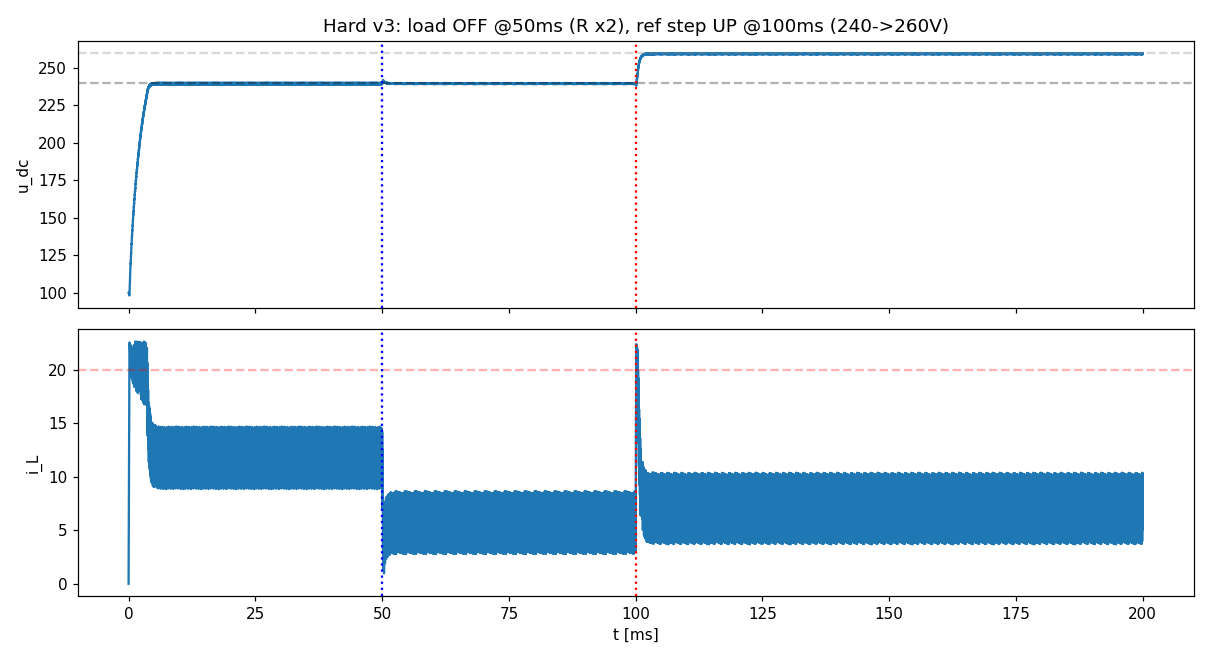
\includegraphics[width=0.95\linewidth]{rysunki/scenario_check.png}
    \caption{Weryfikacja scenariusza trudnego: przebieg napięcia $u_{dc}(t)$ i~prądu cewki $i_L(t)$ dla~ustalonej pary nastaw regulatora. Widoczne dwa zdarzenia: skokowe odciążenie w~$t = 50$~ms oraz skok zadania $240 \to 260$~V w~$t = 100$~ms.}
    \label{fig:scenario-check}
\end{figure}

\subsection{Baseline siatkowy (grid search 15$\times$15)}
\label{subsec:pso-grid}

Przed~uruchomieniem właściwej optymalizacji rojem cząstek przeprowadzono pełną ewaluację siatkową w~przestrzeni $(w_i, f_c)$ na~kracie $15\times 15 = 225$~węzłów, rozmieszczonych równomiernie w~skali logarytmicznej (\texttt{optymalizacja/grid\_search.py}). Granice siatki przyjęto analogicznie do~granic przestrzeni PSO ($w_i\in[0{,}1;\,5]$, $f_c\in[200;\,10\,000]$~Hz). Dla~każdego z~225 węzłów wykonano kompletną symulację scenariusza trudnego oraz~obliczono wszystkie pięć funkcji celu zdefiniowanych w~podrozdziale~\ref{sec:fitness}, otrzymując w~rezultacie pięć dwuwymiarowych map kosztu zobrazowanych na~rysunku~\ref{fig:mapy-kosztow}.

\begin{figure}[h!]
    \centering
    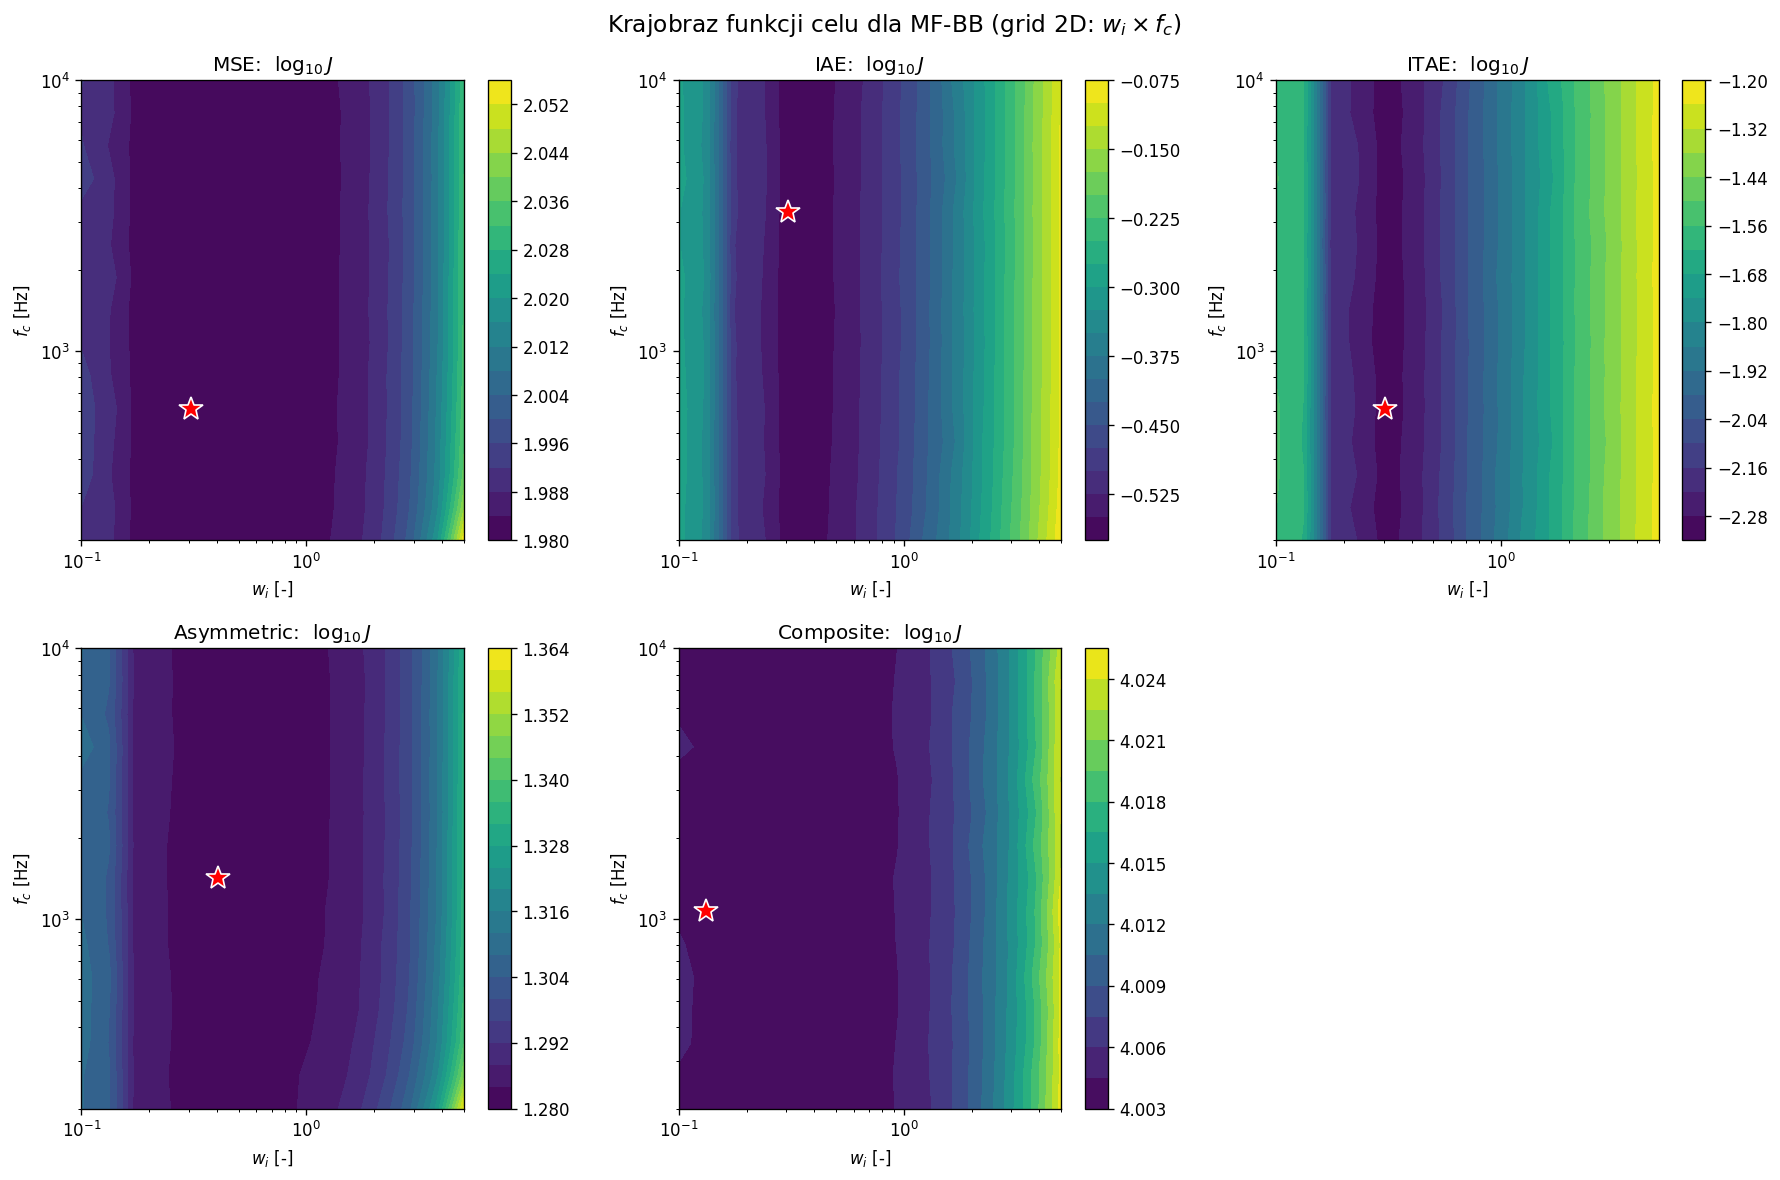
\includegraphics[width=\linewidth]{rysunki/mapy_kosztow.png}
    \caption{Mapy funkcji kosztu w~przestrzeni $(w_i, f_c)$ uzyskane z~grid searcha $15\times 15$ węzłów. Każda mapa odpowiada jednej z~pięciu funkcji celu (MSE, IAE, ITAE, asymetryczna, kompozytowa). Skala logarytmiczna na~obu osiach, krzyżyk oznacza minimum globalne~siatki.}
    \label{fig:mapy-kosztow}
\end{figure}

Baseline siatkowy pełni dwie funkcje. Po~pierwsze, dostarcza punktu odniesienia (\emph{ground truth} w~granicach rozdzielczości kraty) względem~którego można ocenić skuteczność PSO -- algorytm metaheurystyczny powinien znaleźć rozwiązanie nie~gorsze od~najlepszego węzła siatki, zazwyczaj jednak lepsze, gdyż~działa w~przestrzeni ciągłej. Po~drugie, mapy kosztu ujawniają jakościowy charakter krajobrazu optymalizacyjnego -- obecność wielu minimów lokalnych, długich dolin oraz~obszarów płaskich, co~bezpośrednio uzasadnia konieczność użycia metody globalnej zamiast~klasycznych gradientowych. Przebiegi czasowe odpowiadające nastawom optymalnym dla~każdej z~pięciu funkcji celu zestawiono na~rysunku~\ref{fig:przebiegi-optimum}.

\begin{figure}[h!]
    \centering
    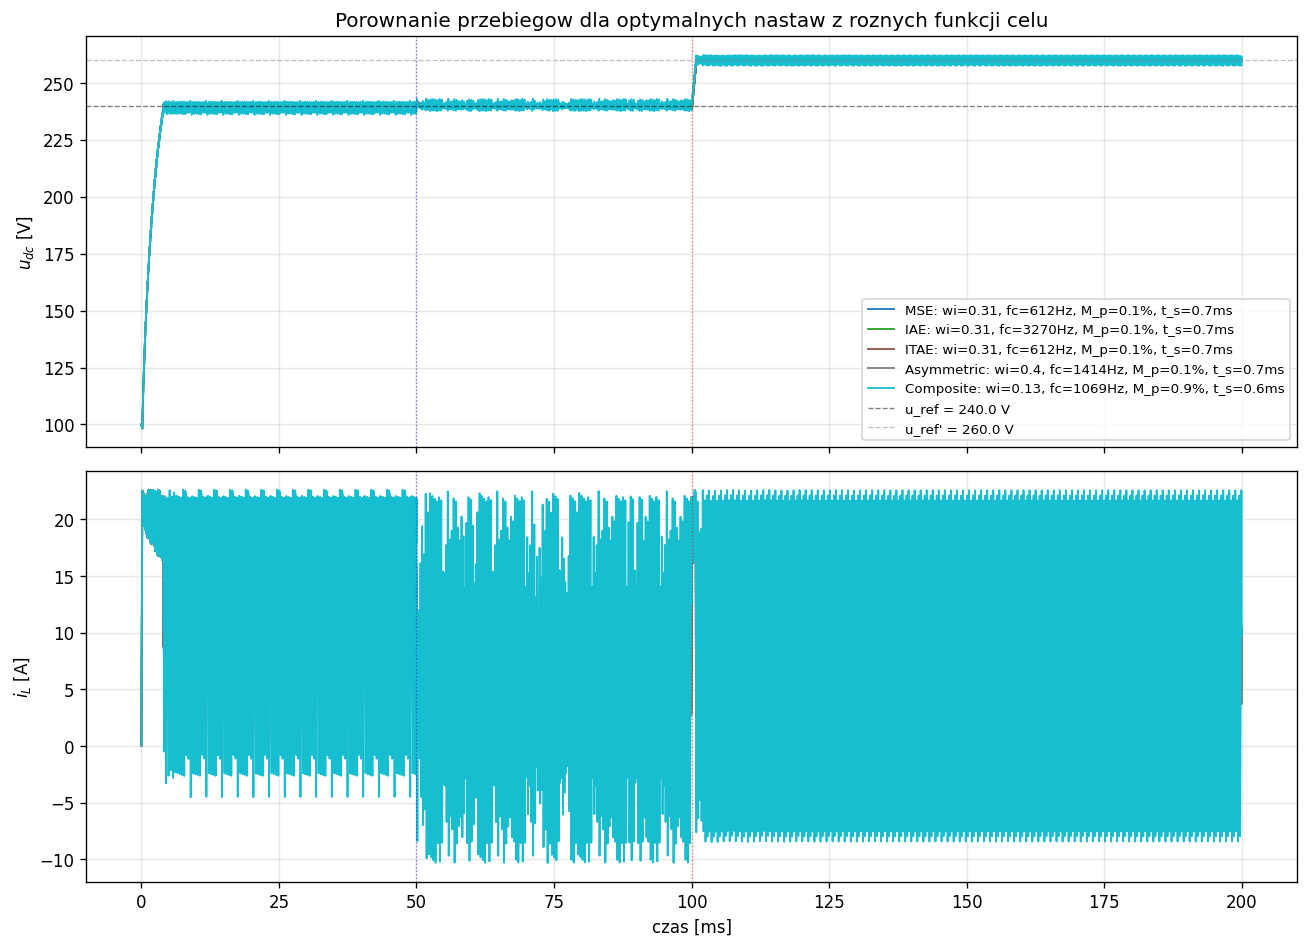
\includegraphics[width=\linewidth]{rysunki/przebiegi_optimum.png}
    \caption{Przebiegi napięcia $u_{dc}(t)$ uzyskane dla~nastaw $(w_i^*,f_c^*)$ minimalizujących każdą z~pięciu funkcji celu na~siatce $15\times 15$. Widoczne jakościowe różnice odpowiedzi -- kryteria całkowe (MSE/IAE/ITAE) faworyzują szybką, agresywną dynamikę, natomiast kryterium asymetryczne i~kompozytowe prowadzą do~odpowiedzi bardziej zachowawczych.}
    \label{fig:przebiegi-optimum}
\end{figure}

\subsection{Pętla ewaluacji w~PSO}
\label{subsec:pso-loop}

Właściwa pętla strojenia jest~realizowana przez~funkcję \texttt{evaluate(log\_wi, log\_fc, cost\_name)} z~modułu \texttt{optymalizacja/pso.py}, której kolejne wywołania PSO wykonuje wewnątrz pętli głównej dla~każdej cząstki w~każdej iteracji. Algorytmiczne kroki pojedynczej ewaluacji są~następujące:
\begin{enumerate}
    \item potęgowanie współrzędnych cząstki: $w_i \leftarrow 10^{\log w_i}$, $f_c \leftarrow 10^{\log f_c}$ (przejście z~przestrzeni PSO do~przestrzeni fizycznej);
    \item podmiana nastaw regulatora w~kopii konfiguracji domyślnej (\texttt{default\_config()}) z~jednoczesnym podpięciem scenariusza trudnego i~horyzontu $T = 200$~ms;
    \item wywołanie metody \texttt{Simulator(cfg).run()} -- pełna symulacja $\sim$$4\cdot 10^{5}$ kroków;
    \item zbudowanie tablicy zadania $u_{\mathrm{ref}}(t)$ uwzględniającej ref-step;
    \item wywołanie funkcji kosztu wybranej z~rejestru \texttt{COST\_FUNCTIONS} i~zwrócenie wartości skalarnej.
\end{enumerate}

Z~perspektywy PSO funkcja \texttt{evaluate} jest~deterministyczną odpowiednikiem czarnej skrzynki -- dla~tych samych argumentów zwraca tę~samą wartość (silnik fizyczny nie~używa generatorów liczb pseudolosowych, a~całe źródło stochastyczności sprowadza się do~inicjalizacji roju przez~\texttt{numpy.random.default\_rng(seed=42)}). Dzięki temu pojedyncze uruchomienie eksperymentu jest~w~pełni powtarzalne, co~ma~kluczowe znaczenie dla~odtwarzalności wyników raportowanych w~rozdziale~\ref{sec:wyniki-pso}.

\section{Wyniki strojenia PSO i~porównanie z~baseline'em}
\label{sec:wyniki-pso}

Algorytm PSO uruchomiono pięciokrotnie -- po~jednym przebiegu na~każdą z~funkcji celu zdefiniowanych w~podrozdziale~\ref{sec:fitness}, przy~tej samej konfiguracji hiperparametrów wymienionych w~tabeli~\ref{tab:pso-hparams} oraz tym samym ziarnie generatora pseudolosowego ($\texttt{seed}=42$). Łączny budżet ewaluacji wyniósł $N\cdot(K_{\max}+1) = 20\cdot 41 = 820$ wywołań silnika fizycznego (kolumna inicjalna~+~$K_{\max}$ iteracji aktualizacji). Wartości optymalnych nastaw $(w_i^*,\,f_c^*)$ wraz z~odpowiadającymi wartościami funkcji celu $J^*$ zestawiono w~tabeli~\ref{tab:pso-wyniki}.

\begin{table}[h!]
    \centering
    \caption{Optymalne nastawy regulatora MF-BB znalezione przez~PSO dla~pięciu funkcji celu (scenariusz trudny, $T = 200$~ms).}
    \label{tab:pso-wyniki}
    \begin{tabular}{lrrr}
        \toprule
        \textbf{Funkcja celu} & $w_i^*$ & $f_c^*$ [Hz] & $J^*$ \\
        \midrule
        MSE        & 0{,}288 & 9569 & $9{,}55\cdot 10^{1}$ \\
        IAE        & 0{,}283 & 2701 & $2{,}69\cdot 10^{-1}$ \\
        ITAE       & 0{,}276 & 9493 & $4{,}71\cdot 10^{-3}$ \\
        Asymetryczna & 0{,}395 & 6902 & $1{,}91\cdot 10^{1}$ \\
        Kompozytowa & 0{,}136 & \phantom{0}618 & $1{,}01\cdot 10^{4}$ \\
        \bottomrule
    \end{tabular}
\end{table}

Pierwsze obserwacje strukturalne dotyczą lokalizacji minimów w~przestrzeni nastaw. Cztery kryteria całkowe (MSE, IAE, ITAE, asymetryczne) wskazują podobny zakres wagi inercji $w_i^* \in [0{,}28;\,0{,}40]$, co~odpowiada umiarkowanej dynamice członu predykcyjnego. Wyróżnia się jedynie kryterium kompozytowe, dla~którego $w_i^* = 0{,}136$ jest~bliskie dolnej granicy przestrzeni przeszukiwań -- regulator preferuje wówczas niemal wyłącznie sygnał błędu, kosztem reakcji predykcyjnej, co~jest~bezpośrednią konsekwencją dominacji składnika $\alpha\cdot t_s$ w~funkcji $J_{\mathrm{Comp}}$ (równanie~\eqref{eq:cost-composite}). Częstotliwość filtru $f_c^*$ jest~znacznie bardziej rozproszona -- od~618~Hz (Composite) do~9569~Hz (MSE), co~odzwierciedla różnicę między~kryteriami penalizującymi pojedyncze szczyty (wymagają agresywnej filtracji, $f_c$~wysokie) a~kryteriami uśredniającymi (tolerują niższe pasmo).

Charakter zbieżności roju dla~poszczególnych funkcji celu pokazano na~rysunku~\ref{fig:pso-zbieznosc-porown}. Wszystkie pięć przebiegów osiągnęło stabilne plateau przed~upływem zadeklarowanego budżetu $K_{\max}=40$ iteracji (ITAE: iteracja~34, Composite: 28, pozostałe: 38--40), co~potwierdza wystarczalność przyjętej konfiguracji. Charakterystyczne stopniowe spadki w~początkowych iteracjach odpowiadają pierwszym odkryciom obszarów obiecujących przez~poszczególne cząstki, natomiast późniejsza monotoniczna zbieżność wynika z~liniowej dekrementacji wagi bezwładności (równanie~\eqref{eq:pso-inertia}).

\begin{figure}[h!]
    \centering
    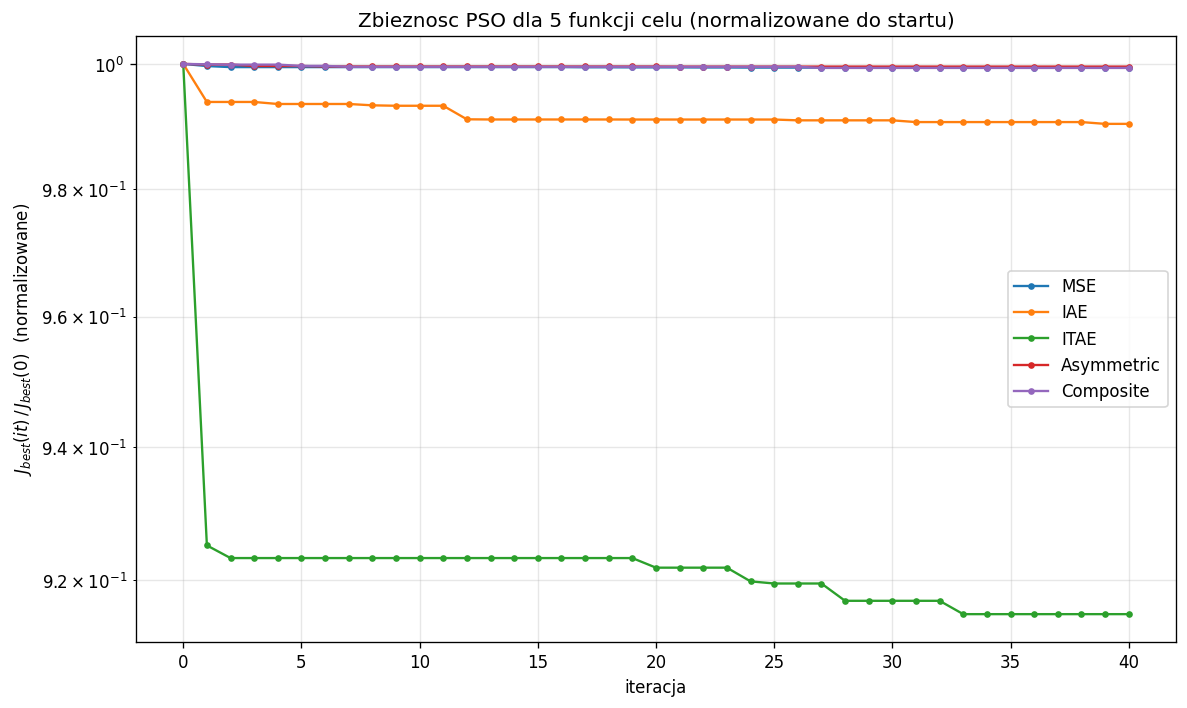
\includegraphics[width=\linewidth]{rysunki/pso_porownanie_zbieznosci.png}
    \caption{Krzywe zbieżności PSO dla~pięciu funkcji celu w~funkcji numeru iteracji. Każda krzywa znormalizowana do~swojej wartości początkowej ($J^{(0)}/J^{(0)}=1$); skala logarytmiczna podkreśla ostatnie rzędy poprawy.}
    \label{fig:pso-zbieznosc-porown}
\end{figure}

Wizualizację samego procesu przeszukiwania przedstawia rysunek~\ref{fig:pso-roj}, na~którym kolejne pozycje wszystkich cząstek roju zostały naniesione na~mapę funkcji kosztu uzyskaną z~grid searcha. Dla~każdej z~pięciu funkcji celu obserwuje się charakterystyczne kondensowanie się chmury cząstek wokół minimum w~ciągu pierwszych 10--15 iteracji, po~czym następuje faza dokładnej lokalnej eksploracji w~zwartym obszarze.

\begin{figure}[h!]
    \centering
    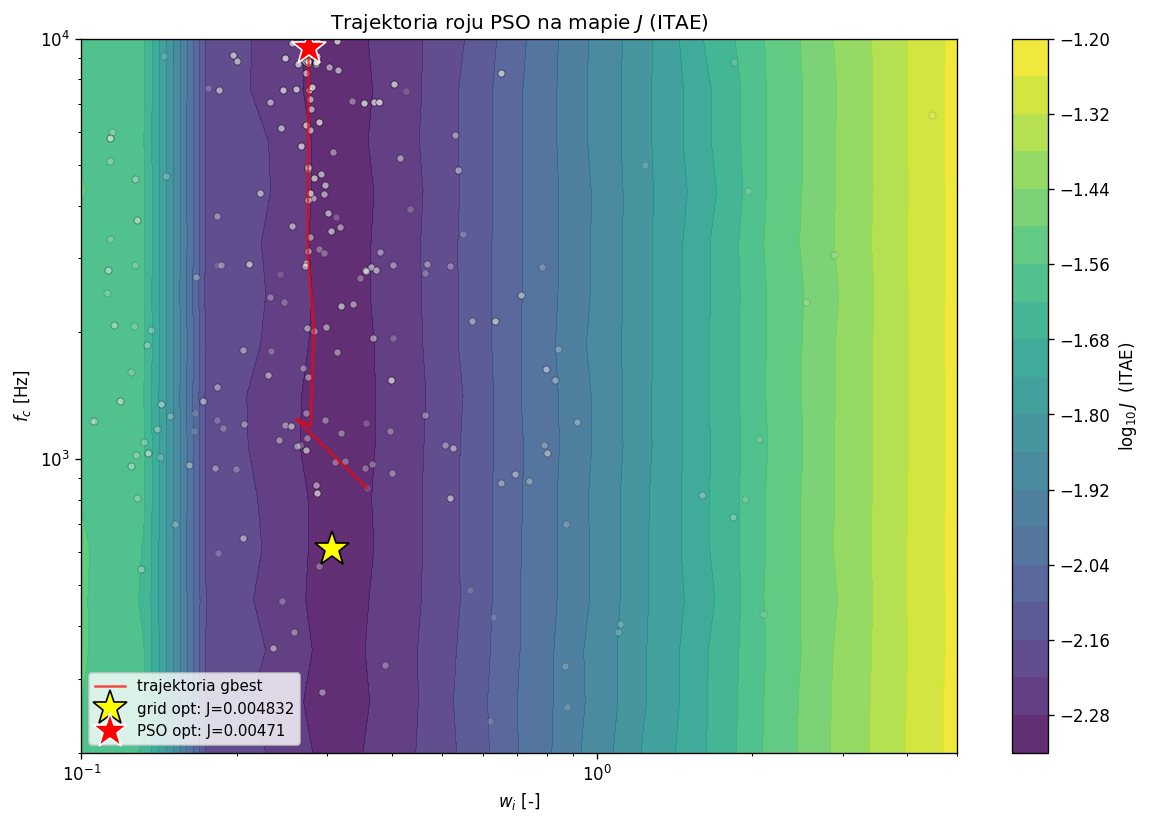
\includegraphics[width=\linewidth]{rysunki/pso_roj_na_mapie.png}
    \caption{Trajektoria roju cząstek PSO nałożona na~mapę funkcji kosztu (grid search 15$\times$15) dla~pięciu funkcji celu. Kolory cząstek odpowiadają numerowi iteracji (gradient od~jasnego do~ciemnego), gwiazda oznacza znalezione $\mathbf{g}^*$.}
    \label{fig:pso-roj}
\end{figure}

\subsection{Porównanie ilościowe PSO vs.~grid search}
\label{subsec:pso-vs-grid}

Bezpośrednie zestawienie wartości funkcji celu osiągniętych przez~PSO i~przez~najlepszy węzeł siatki bazowej (225~symulacji) przedstawia rysunek~\ref{fig:pso-vs-grid}. PSO uzyskuje wartości funkcji celu nie~gorsze od~baseline'u siatkowego dla~wszystkich pięciu kryteriów, przy~czym największą poprawę odnotowano dla~kryterium ITAE: wartość $J^*_{\mathrm{PSO}} = 4{,}71\cdot 10^{-3}$ jest~o~ok.~2{,}5\% niższa od~minimum siatkowego $J^*_{\mathrm{grid}} = 4{,}83\cdot 10^{-3}$. Dla~pozostałych kryteriów różnica jest~marginalna (poniżej~0{,}3\%), co~należy interpretować jako~potwierdzenie, że~siatka 15$\times$15 trafiła blisko prawdziwego optimum, a~PSO dokończył eksplorację w~przestrzeni ciągłej.

\begin{figure}[h!]
    \centering
    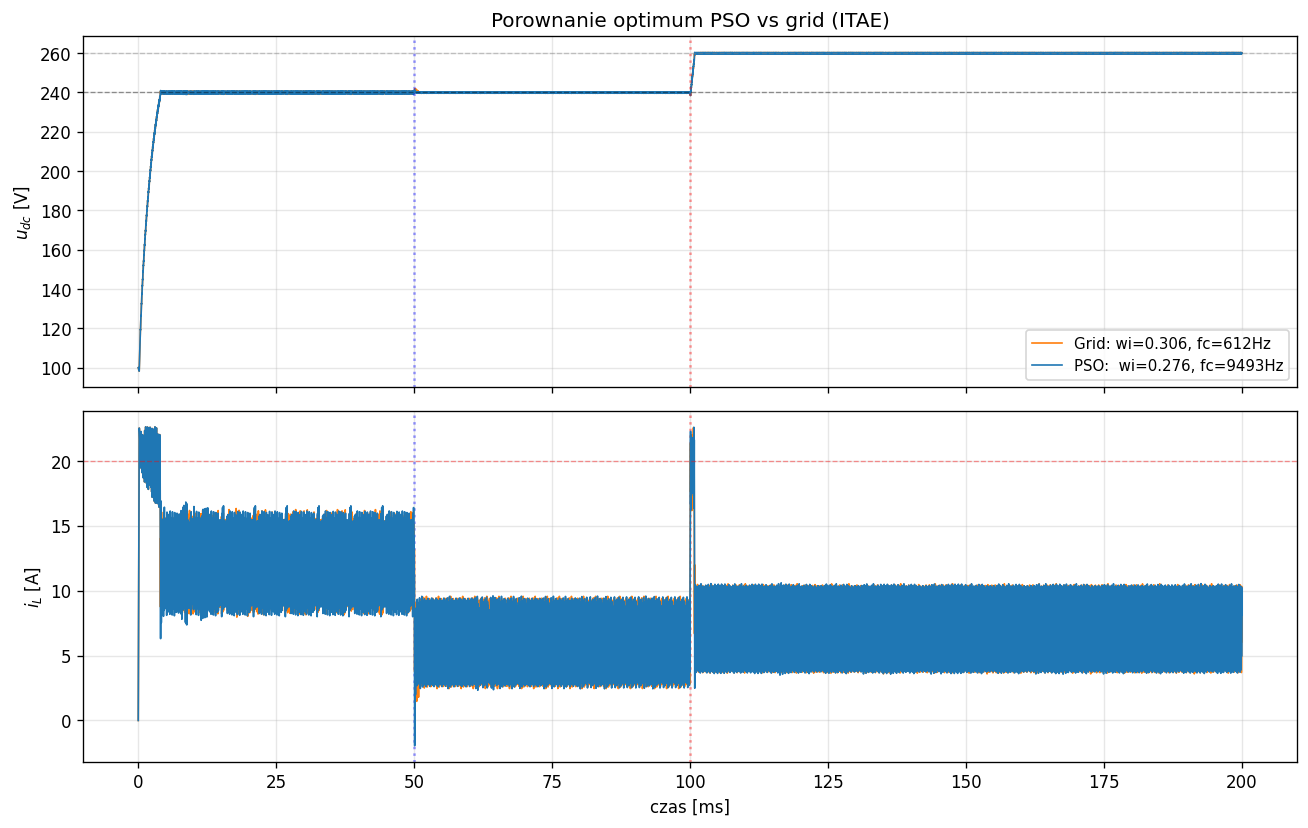
\includegraphics[width=0.85\linewidth]{rysunki/pso_vs_grid.png}
    \caption{Porównanie wartości funkcji celu $J^*$ uzyskanej przez~PSO (820~ewaluacji) z~minimum siatki 15$\times$15 (225~ewaluacji) dla~pięciu kryteriów. Wartości znormalizowane do~minimum grid (=1{,}00); PSO poniżej~1 oznacza lepszy wynik.}
    \label{fig:pso-vs-grid}
\end{figure}

Z~perspektywy efektywności obliczeniowej PSO osiągnął porównywalne wyniki przy~3,6-krotnie większej liczbie ewaluacji (820 vs.~225). Przewaga metaheurystyki ujawnia się jednak dopiero przy~rozszerzeniu wymiaru przestrzeni przeszukiwań -- dla~regulatora z~$d=4$ hiperparametrami (np.~dodanie współczynników predyktora) siatka tej~samej rozdzielczości wymagałaby $15^4 = 50\,625$ symulacji, podczas gdy PSO zachowuje liniową złożoność $\mathcal{O}(N\cdot K_{\max})$ niezależnie od~$d$.

Jakościowe porównanie wpływu wyboru funkcji celu na~odpowiedź czasową regulatora przedstawia rysunek~\ref{fig:pso-przebiegi}. Widoczne są~istotne różnice charakteru regulacji: kryterium kompozytowe prowadzi do~zauważalnego undershoot po~skoku zadania (skutek dominacji $\alpha\cdot t_s$), kryterium asymetryczne praktycznie eliminuje przeregulowanie kosztem dłuższego czasu ustalania, natomiast kryteria MSE/IAE/ITAE generują odpowiedzi zbliżone jakościowo, z~niewielkim przeregulowaniem rzędu kilku~procent.

\begin{figure}[h!]
    \centering
    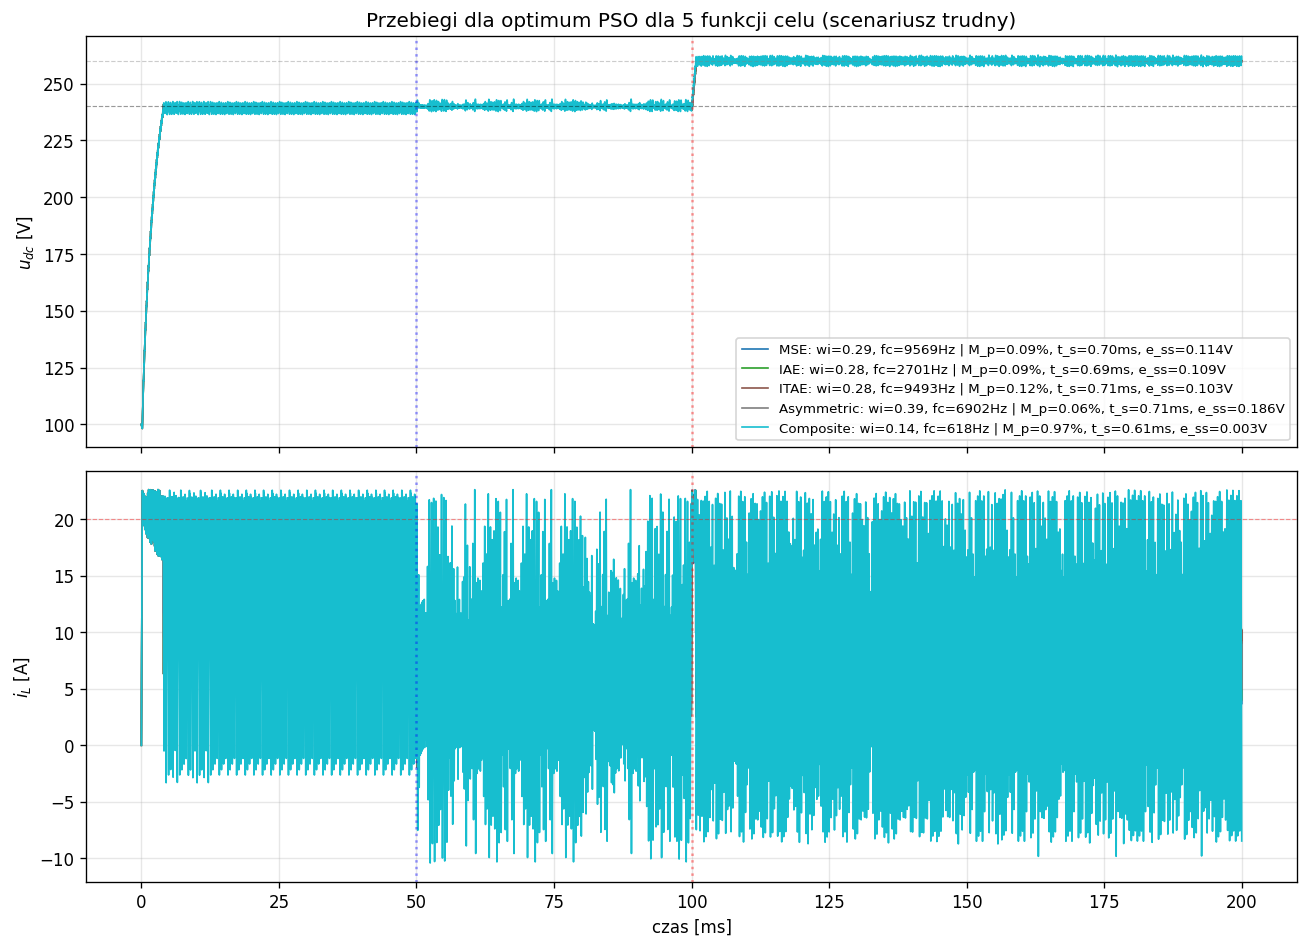
\includegraphics[width=\linewidth]{rysunki/pso_porownanie_przebiegow.png}
    \caption{Odpowiedzi napięciowe regulatora MF-BB nastrojonego przez~PSO dla~pięciu funkcji celu w~scenariuszu trudnym. Linia przerywana oznacza zadane $u_{\mathrm{ref}}(t)$.}
    \label{fig:pso-przebiegi}
\end{figure}

Powyższe porównanie potwierdza, że~dobór funkcji celu jest~istotniejszy dla~ostatecznego charakteru regulacji niż~sam wybór algorytmu metaheurystycznego -- pięć przebiegów PSO o~identycznej konfiguracji algorytmu zwróciło pięć jakościowo różnych nastaw regulatora, każdy optymalny w~sensie swojego kryterium.

\subsection{Optymalizacja wielokryterialna w~scenariuszu dynamicznym i~redukcja tętnień prądu}
\label{subsec:pso-dynamic-scenario}

W~celu ostatecznej weryfikacji zdolności algorytmu PSO do~równoważenia jakości regulacji napięcia oraz redukcji tętnień prądu cewki, przeprowadzono optymalizację w~złożonym scenariuszu dynamicznym o~horyzoncie $T_{\mathrm{end}} = 0{,}30~\mathrm{s}$. Obiekt badawczy skonfigurowano dla parametrów: $V_{\mathrm{in}} = 100~\mathrm{V}$, $L = 0{,}75~\mathrm{mH}$ ($750~\mu\mathrm{H}$), $C = 200~\mu\mathrm{F}$ oraz znamionowego obciążenia $R_{\mathrm{load}} = 47{,}619~\Omega$ (co odpowiada mocy znamionowej $P \approx 1{,}2~\mathrm{kW}$ przy napięciu $240~\mathrm{V}$).

Scenariusz obejmuje sekwencję głębokich zaburzeń stanu pracy:
\begin{enumerate}
    \item $t \in [0;\, 50)~\mathrm{ms}$ -- rozruch układu od napięcia $u_{dc}(0) = 100~\mathrm{V}$ do poziomu zadanego $u_{\mathrm{ref}} = 240~\mathrm{V}$;
    \item $t = 50~\mathrm{ms}$ -- nagłe zrzucenie obciążenia ($R_{\mathrm{load}} \leftarrow 10~\mathrm{M}\Omega$, stan jałowy / rozwarcie obwodu wyjściowego);
    \item $t = 100~\mathrm{ms}$ -- ponowne załączenie nominalnego odbiornika $R_{\mathrm{load}} \leftarrow 47{,}619~\Omega$;
    \item $t = 150~\mathrm{ms}$ -- skok napięcia zadanego w~dół: $u_{\mathrm{ref}} \leftarrow 160~\mathrm{V}$;
    \item $t = 200~\mathrm{ms}$ -- powtórne odłączenie obciążenia ($R_{\mathrm{load}} \leftarrow 10~\mathrm{M}\Omega$);
    \item $t = 250~\mathrm{ms}$ -- powrót do pełnego obciążenia przy obniżonym napięciu wyjściowym;
    \item $t = 300~\mathrm{ms}$ -- zakończenie cyklu testowego.
\end{enumerate}

Dla opisanego scenariusza wykonano optymalizację PSO nastaw regulatora $\mathbf{x} = [w_i, f_c]$ z~uwzględnieniem modelowej korekty opóźnienia próbkowania. Porównano cztery warianty funkcji celu: kryterium bazowe oparte wyłącznie na błędzie napięcia (ITAE) oraz trzy kryteria świadome prądu (CurrentAware, CurrentOscillation, CurrentEffort) zdefiniowane w~podrozdziale~\ref{subsec:cost-current}. Znalezione przez algorytm optymalne wektory nastaw zestawiono w~tabeli~\ref{tab:pso-dynamic-opt}.

\begin{table}[h!]
    \centering
    \caption{Optymalne nastawy regulatora znalezione przez PSO w~scenariuszu dynamicznym ($T_{\mathrm{end}} = 0{,}30~\mathrm{s}$).}
    \label{tab:pso-dynamic-opt}
    \begin{tabular}{lrrr}
        \toprule
        \textbf{Funkcja celu} & $w_i^*$ & $f_c^*$ [Hz] & $J^*$ \\
        \midrule
        ITAE (odniesienie)         & 0{,}2133 & 1854 & $1{,}58\cdot 10^{-2}$ \\
        CurrentAware (Wariant 1)     & 0{,}2631 & 7056 & $5{,}60\cdot 10^{-1}$ \\
        CurrentOscillation (Wariant 2)& 0{,}2124 & 2039 & $4{,}15\cdot 10^{-1}$ \\
        CurrentEffort (Wariant 3)    & 0{,}2131 & 2767 & $7{,}16\cdot 10^{-1}$ \\
        \bottomrule
    \end{tabular}
\end{table}

Kluczowym elementem analizy jest ilościowa ocena jakości pracy w~stanach ustalonych pomiędzy komutacjami obciążenia i~skokami referencji. Wskaźniki jakości wyznaczono z~okna obejmującego ostatnie 40\,\% czasu trwania każdego z~segmentów, co eliminuje wpływ stanów przejściowych. Zestawienie metryk zawiera tabela~\ref{tab:scenariusz-metryki}.

\begin{table}[h!]
    \centering
    \small
    \caption{Zestawienie wskaźników w~stanach ustalonych (ostatnie 40\,\% każdego segmentu) dla czterech wariantów nastrojonych przez PSO.}
    \label{tab:scenariusz-metryki}
    \begin{tabular}{lrrrrr}
        \toprule
        \textbf{Segment} & $u_{\mathrm{ref}}$~[V] & $e_u$~[V] & $\bar{i}_L$~[A] & $\Delta i_{L,\mathrm{pp}}$~[A] & Tętnienia [\%] \\
        \midrule
        \multicolumn{6}{l}{\textbf{ITAE (odniesienie: $w_i^* = 0{,}2133$, $f_c^* = 1854$~Hz)}} \\
        $[0{,}05;\, 0{,}10)$~s (OFF) & 240{,}0 & $-0{,}11$ & $-0{,}05$ & 3{,}43 & --- \\
        $[0{,}10;\, 0{,}15)$~s (ON)  & 240{,}0 & $-0{,}29$ & 12{,}10 & 5{,}70 & 47{,}12 \\
        $[0{,}15;\, 0{,}20)$~s (ON)  & 160{,}0 & $+0{,}17$ & 5{,}38 & 3{,}45 & 64{,}01 \\
        $[0{,}20;\, 0{,}25)$~s (OFF) & 160{,}0 & $+0{,}12$ & $-0{,}02$ & 2{,}35 & --- \\
        $[0{,}25;\, 0{,}30)$~s (ON)  & 160{,}0 & $+0{,}17$ & 5{,}38 & 2{,}62 & 48{,}71 \\
        \midrule
        \multicolumn{6}{l}{\textbf{CurrentAware (Wariant 1: $w_i^* = 0{,}2631$, $f_c^* = 7056$~Hz)}} \\
        $[0{,}05;\, 0{,}10)$~s (OFF) & 240{,}0 & $-0{,}14$ & $-0{,}05$ & 3{,}41 & --- \\
        $[0{,}10;\, 0{,}15)$~s (ON)  & 240{,}0 & $-0{,}35$ & 12{,}09 & \textbf{3{,}73} & \textbf{30{,}83} \\
        $[0{,}15;\, 0{,}20)$~s (ON)  & 160{,}0 & $+0{,}20$ & 5{,}38 & 2{,}61 & 48{,}39 \\
        $[0{,}20;\, 0{,}25)$~s (OFF) & 160{,}0 & $+0{,}14$ & $-0{,}02$ & 2{,}34 & --- \\
        $[0{,}25;\, 0{,}30)$~s (ON)  & 160{,}0 & $+0{,}20$ & 5{,}38 & 2{,}55 & 47{,}28 \\
        \midrule
        \multicolumn{6}{l}{\textbf{CurrentOscillation (Wariant 2: $w_i^* = 0{,}2124$, $f_c^* = 2039$~Hz)}} \\
        $[0{,}05;\, 0{,}10)$~s (OFF) & 240{,}0 & $-0{,}11$ & $-0{,}05$ & 3{,}43 & --- \\
        $[0{,}10;\, 0{,}15)$~s (ON)  & 240{,}0 & $-0{,}29$ & 12{,}09 & 6{,}80 & 56{,}24 \\
        $[0{,}15;\, 0{,}20)$~s (ON)  & 160{,}0 & $+0{,}17$ & 5{,}38 & 3{,}47 & 64{,}45 \\
        $[0{,}20;\, 0{,}25)$~s (OFF) & 160{,}0 & $+0{,}12$ & $-0{,}02$ & 2{,}33 & --- \\
        $[0{,}25;\, 0{,}30)$~s (ON)  & 160{,}0 & $+0{,}17$ & 5{,}38 & 3{,}45 & 64{,}10 \\
        \midrule
        \multicolumn{6}{l}{\textbf{CurrentEffort (Wariant 3: $w_i^* = 0{,}2131$, $f_c^* = 2767$~Hz)}} \\
        $[0{,}05;\, 0{,}10)$~s (OFF) & 240{,}0 & $-0{,}11$ & $-0{,}05$ & 3{,}42 & --- \\
        $[0{,}10;\, 0{,}15)$~s (ON)  & 240{,}0 & $-0{,}29$ & 12{,}10 & 5{,}70 & 47{,}09 \\
        $[0{,}15;\, 0{,}20)$~s (ON)  & 160{,}0 & $+0{,}17$ & 5{,}38 & 3{,}45 & 64{,}10 \\
        $[0{,}20;\, 0{,}25)$~s (OFF) & 160{,}0 & $+0{,}12$ & $-0{,}02$ & 2{,}37 & --- \\
        $[0{,}25;\, 0{,}30)$~s (ON)  & 160{,}0 & $+0{,}17$ & 5{,}38 & 3{,}45 & 64{,}12 \\
        \bottomrule
    \end{tabular}
\end{table}

Pełne przebiegi czasowe napięcia i~prądu dla wszystkich czterech wariantów w~horyzoncie $0{,}30~\mathrm{s}$ przedstawiono na~rysunku~\ref{fig:scenariusz-prof-pelny}, natomiast zbliżenie w~pełnej rozdzielczości próbek ($0{,}5~\mu\mathrm{s}$) w~oknie $140$--$210~\mathrm{ms}$ (obejmujące skok wartości zadanej $240 \to 160~\mathrm{V}$ oraz wyłączenie obciążenia) zilustrowano na~rysunku~\ref{fig:scenariusz-prof-zoom}.

\begin{figure}[h!]
    \centering
    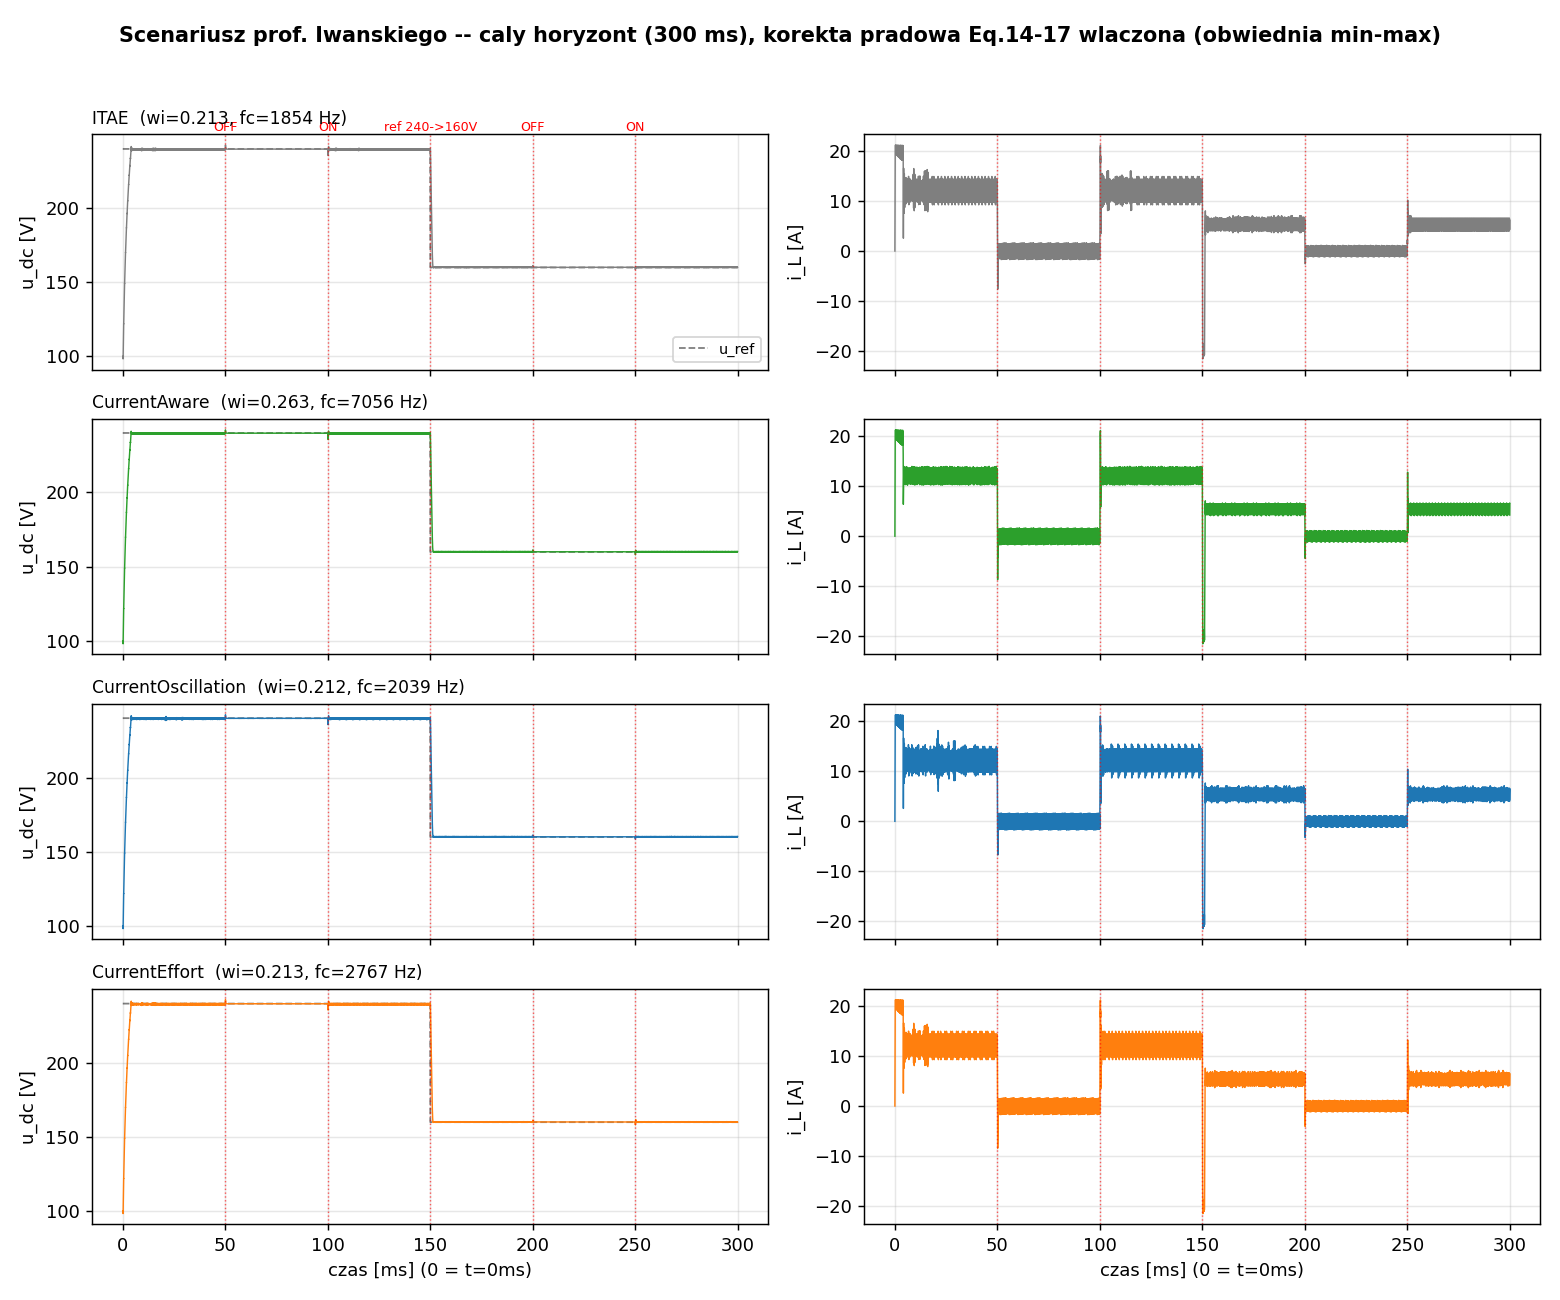
\includegraphics[width=\linewidth]{rysunki/wykres_scenariusz_prof_pelny.png}
    \caption{Przebiegi napięcia wyjściowego $u_{dc}(t)$ oraz prądu dławika $i_L(t)$ dla czterech wariantów funkcji celu w~scenariuszu dynamicznym ($T_{\mathrm{end}} = 0{,}30~\mathrm{s}$, linie przerywane wskazują momenty komutacji obciążenia i~skoku referencji).}
    \label{fig:scenariusz-prof-pelny}
\end{figure}

\begin{figure}[h!]
    \centering
    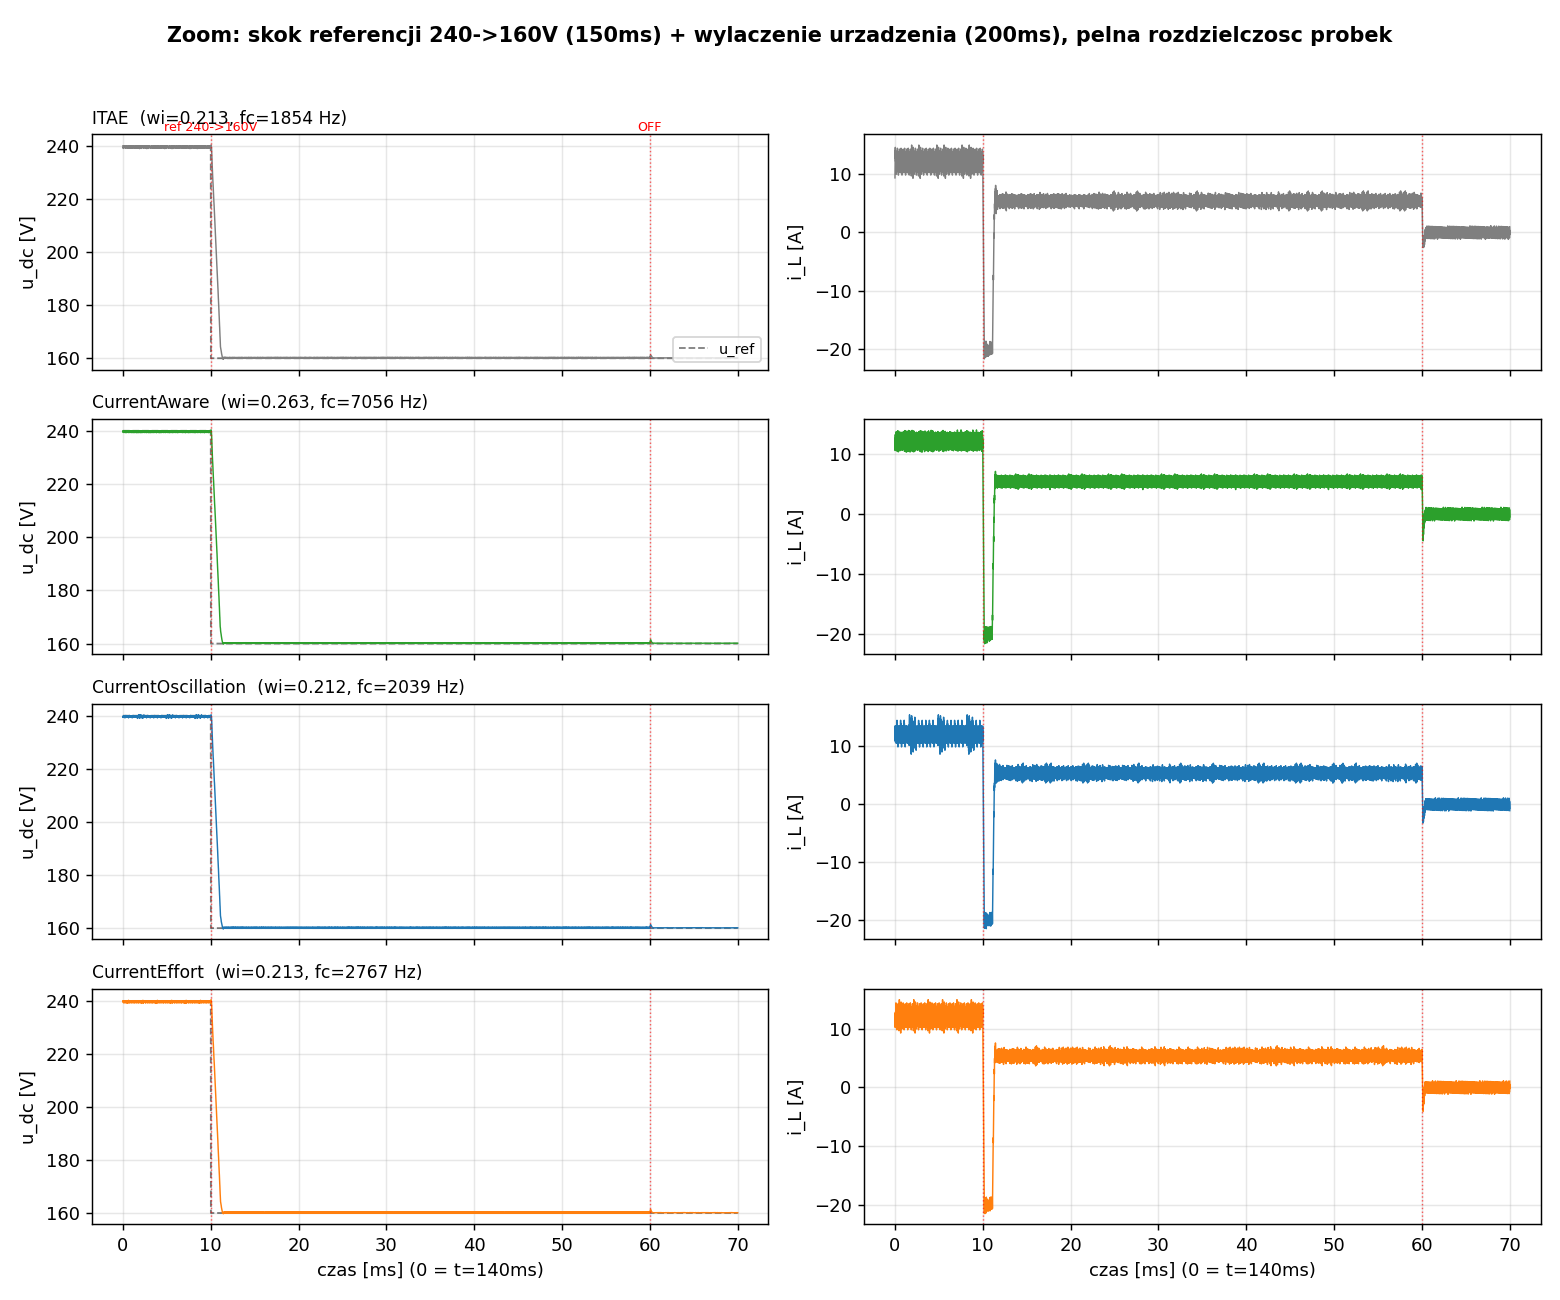
\includegraphics[width=\linewidth]{rysunki/wykres_scenariusz_prof_zoom.png}
    \caption{Zbliżenie mikrosekundowe (okno $140$--$210~\mathrm{ms}$, pełna rozdzielczość próbek $0{,}5~\mu\mathrm{s}$) ilustrujące skok napięcia zadanego w~$t=150~\mathrm{ms}$ oraz zrzucenie obciążenia w~$t=200~\mathrm{ms}$.}
    \label{fig:scenariusz-prof-zoom}
\end{figure}

Analiza uzyskanych wyników prowadzi do~trzech zasadniczych wniosków:
\begin{enumerate}
    \item \textbf{Wysoka precyzja regulacji napięcia we wszystkich wariantach:} średni błąd napięcia w~stanie ustalonym mieści się w~wąskim przedziale od~$-0{,}35~\mathrm{V}$ do~$+0{,}20~\mathrm{V}$ (błąd względny poniżej $0{,}15\,\%$), a~średni prąd cewki idealnie realizuje teoretyczny bilans mocy: $\bar{i}_L \approx 12{,}09~\mathrm{A}$ dla $240~\mathrm{V}$ ($1{,}2~\mathrm{kW}$) oraz $\bar{i}_L \approx 5{,}38~\mathrm{A}$ dla $160~\mathrm{V}$ ($538~\mathrm{W}$).
    \item \textbf{Wyraźna redukcja tętnień prądu w~wariancie CurrentAware:} algorytm PSO dla funkcji celu $J_{\mathrm{CA}}$ dobrał wyższą wagę prądu $w_i^* = 0{,}2631$ oraz znacznie szersze pasmo filtru $f_c^* = 7056~\mathrm{Hz}$. Skutkiem tego amplituda tętnień prądu w~stanie ustalonym pod pełnym obciążeniem ($240~\mathrm{V}$) spadła z~$5{,}70~\mathrm{A}$ ($47{,}12\,\%$ w~ITAE) do~$3{,}73~\mathrm{A}$ ($30{,}83\,\%$). Oznacza to~zmniejszenie rozstępu tętnień prądu o~aż~$34{,}6\,\%$ bez utraty stabilności i~bez widocznego pogorszenia dynamiki napięcia.
    \item \textbf{Strukturalna natura tętnień prądu:} warianty CurrentOscillation i~CurrentEffort zbiegły do~nastaw niemal identycznych jak bazowe ITAE ($w_i^* \approx 0{,}213$, $f_c^* \approx 2000$--$2700~\mathrm{Hz}$). Wynika to~z~faktu, że~dolna granica tętnień jest uwarunkowana sprzętowo przez indukcyjność $L$ i~częstotliwość komutacji ($\Delta i_L \approx \frac{V_{\mathrm{in}} D T_{\mathrm{sw}}}{L}$). Człon prądowy w~funkcji celu działa jako bariera odrzucająca patologiczne nastawy regulatora, pozwalając algorytmowi AI osiągnąć fizyczną dolną granicę tętnień dopuszczalną w~danym układzie.
\end{enumerate}

\subsection{Dwuetapowa procedura optymalizacji regulatora Trend MF-BB}
\label{subsec:pso-two-stage}

Obserwacja dynamiki regulatora przy zredukowanej pojemności wyjściowej ($C = 200~\mu\mathrm{F}$) ujawniła, że podczas gwałtownego skoku napięcia zadanego w dół ($240 \to 160~\mathrm{V}$ w $t = 150~\mathrm{ms}$) klasyczna struktura MF-BB wykazuje skłonność do zapadu napięcia poniżej wartości zadanej (undershoot rzędu $\sim 7$--$8~\mathrm{V}$). Wynika to z faktu, że przy skoku w dół prąd dławika wchodzi w ujemne nasycenie ogranicznika prądowego ($I_{\min} = -20~\mathrm{A}$), a sam uchyb napięcia nie dostarcza sterownikowi informacji o prędkości zbliżania się do nowego punktu pracy.

W celu eliminacji tego zjawiska zastosowano rozszerzoną strukturę regulatora Trend MF-BB z filtrowanym trendem napięcia wyjściowego:
\begin{equation}
    e_{\mathrm{BB}}(k) = \bigl(u_{\mathrm{ref}}(k) - u_{\mathrm{out}}(k)\bigr) + w_i \cdot \bigl(i_{\mathrm{des}}(k) - i_L(k)\bigr) - w_u \cdot \Delta u_f(k),
    \label{eq:trend-mfbb-surface}
\end{equation}
gdzie $\Delta u_f(k) = u_f(k) - u_f(k-1)$ jest przyrostem napięcia wyjściowego przefiltrowanego dyskretnym filtrem dolnoprzepustowym 1. rzędu o częstotliwości odcięcia $f_{c,u}$, a $w_u$ stanowi wagę dynamicznego tłumienia.

Zgodnie z wytycznymi metodycznymi, proces doboru parametrów wektora $\mathbf{x} = [w_i, f_{c,i}, w_u, f_{c,u}]$ zrealizowano w sposób ściśle dwutorowy (decoupled two-stage optimization), rozdzielając optymalizację stanu ustalonego od optymalizacji stanu przejściowego:

\begin{enumerate}
    \item \textbf{Krok 1 -- Stan ustalony ($w_u = 0$):} W stanie ustalonym napięcie wyjściowe nie wykazuje trendu ($\Delta u_f \approx 0$). Przyjmując $w_u = 0$, algorytm PSO dobiera parę $(w_i^*, f_{c,i}^*)$ w oknie ustalonej pracy pod obciążeniem $1{,}2~\mathrm{kW}$ ($t \in [120;\, 150]~\mathrm{ms}$), minimalizując ważoną sumę odchyłki napięcia i błędu śledzenia prądu:
    \begin{equation}
        J_1(w_i, f_{c,i}) = \mathrm{IAE}_u + \lambda_i \cdot \mathrm{IAE}_i = \frac{1}{N}\sum |u_{\mathrm{dc}} - 240\,\mathrm{V}| + \lambda_i \cdot \frac{1}{N}\sum |i_{\mathrm{des}} - i_L|,
        \label{eq:cost-step1}
    \end{equation}
    gdzie współczynnik $\lambda_i$ określa relację wagową błąd napięcia vs. błąd prądu.
    \item \textbf{Krok 2 -- Stan przejściowy (zamrożone parametry z Kroku 1):} Mając ustalone i zamrożone wartości $(w_i^*, f_{c,i}^*)$, algorytm optymalizuje parametry dynamicznego tłumienia $(w_u^*, f_{c,u}^*)$ w oknie skoku napięcia $240 \to 160~\mathrm{V}$ ($t \in [150;\, 165]~\mathrm{ms}$). Zgodnie z zasadami teorii sterowania, stan nasycenia prądu ($i_L \le -20~\mathrm{A}$) nie podlega optymalizacji (steruje nim nadrzędny ogranicznik sprzętowy). Funkcja celu transjentu łączy całkę kwadratu błędu (kryterium ISE) z karą za zapad poniżej linii $160~\mathrm{V}$:
    \begin{equation}
        J_2(w_u) = \int_{150\,\mathrm{ms}}^{165\,\mathrm{ms}} \bigl(u_{\mathrm{dc}}(t) - 160\,\mathrm{V}\bigr)^2\, dt + w_{\mathrm{cross}} \cdot \bigl(\Delta U_{\mathrm{undershoot}}\bigr)^2,
        \label{eq:cost-step2}
    \end{equation}
    gdzie $\Delta U_{\mathrm{undershoot}} = \max\bigl(0,\, 160{,}0\,\mathrm{V} - \min_{t \in [150;\, 155]\,\mathrm{ms}} u_{\mathrm{dc}}(t)\bigr)$, a $w_{\mathrm{cross}}$ jest współczynnikiem kary za zapad (nominalnie $w_{\mathrm{cross}} = 0{,}10$).
\end{enumerate}

Dla nominalnych parametrów filtrów przyjętych z modelu fizycznego i publikacji IEEE ($f_{c,i} = f_{c,u} = 321{,}0~\mathrm{Hz}$, co dla $T_s = 10~\mu\mathrm{s}$ odpowiada współczynnikom Tustina $\alpha = 0{,}0100$, $\beta = 0{,}9800$), procedura dwuetapowa zwróciła nastawy:
\begin{equation}
    w_i^* = 0{,}4000, \quad w_u^* = 15{,}00, \quad f_{c,i} = f_{c,u} = 321{,}0~\mathrm{Hz}.
    \label{eq:optimal-settings-nominal}
\end{equation}
Wartość $w_i^* = 0{,}40$ zapewnia bezpieczny margines stabilności powyżej granicy oscylacji podharmonicznych ($w_i \approx 0{,}25$), natomiast $w_u^* = 15{,}0$ redukuje zapad napięcia po skoku z $7{,}05~\mathrm{V}$ do zaledwie $0{,}26~\mathrm{V}$ (redukcja o $96{,}3\,\%$) bez jakiegokolwiek odbicia w górę.

Odpowiedź czasową układu dla nastaw~\eqref{eq:optimal-settings-nominal} przedstawiono na rysunku~\ref{fig:wykres-dwuetapowy-pelny} (pełny horyzont $0$--$300~\mathrm{ms}$) oraz na rysunku~\ref{fig:wykres-dwuetapowy-zoom} (zbliżenie okna $140$--$210~\mathrm{ms}$ w pełnej rozdzielczości próbek $0{,}5~\mu\mathrm{s}$).

\begin{figure}[h!]
    \centering
    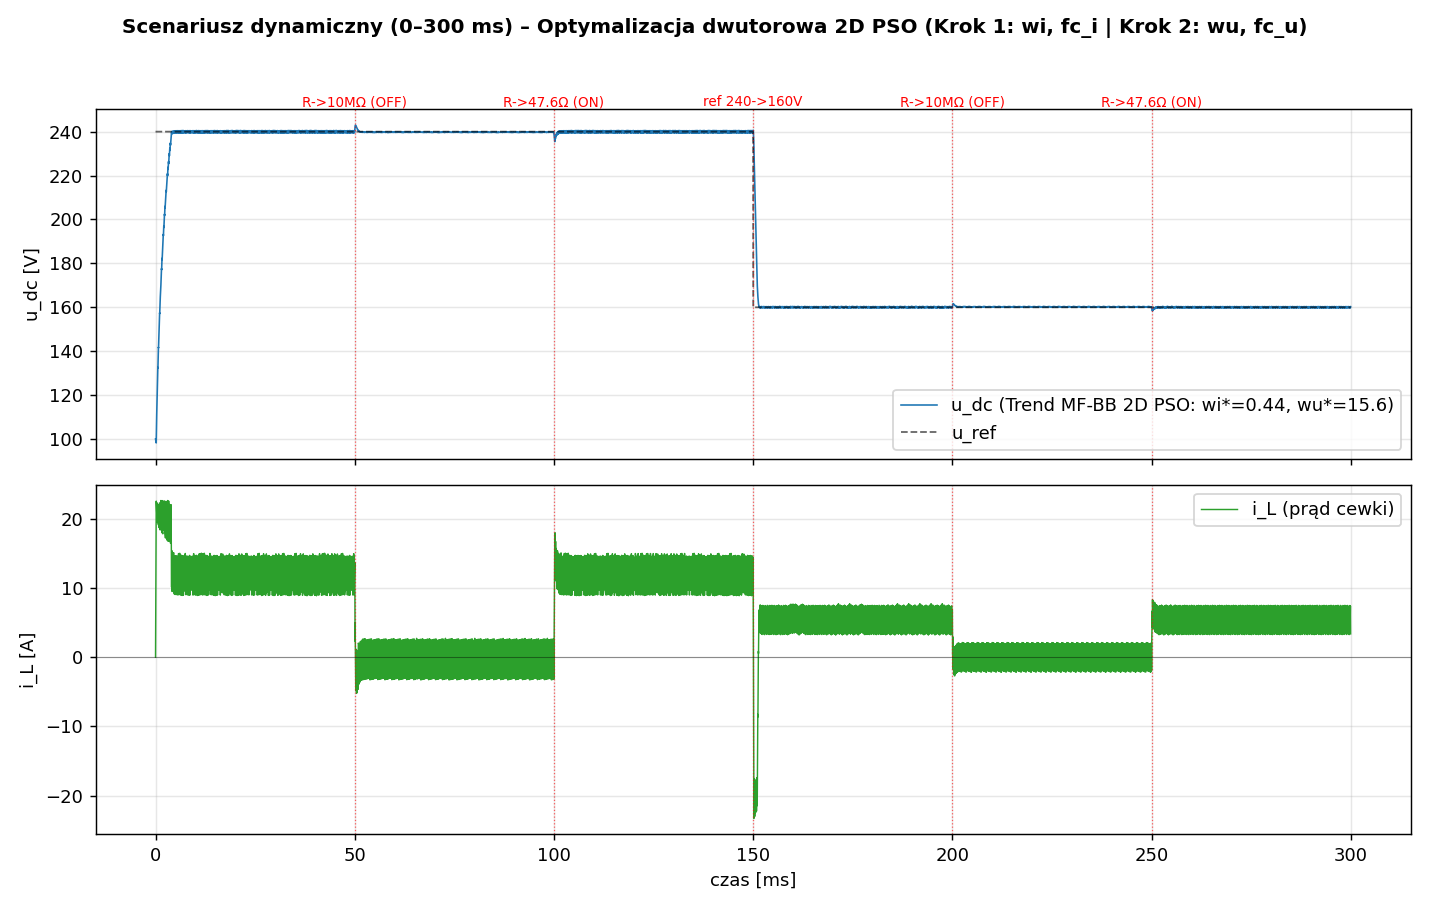
\includegraphics[width=\linewidth]{rysunki/wykres_dwuetapowy_pelny.png}
    \caption{Przebiegi napięcia wyjściowego $u_{\mathrm{dc}}(t)$ oraz prądu cewki $i_L(t)$ dla regulatora Trend MF-BB z nastawami wyznaczonymi procedurą dwuetapową ($w_i^* = 0{,}40$, $w_u^* = 15{,}0$, $f_c = 321{,}0~\mathrm{Hz}$).}
    \label{fig:wykres-dwuetapowy-pelny}
\end{figure}

\begin{figure}[h!]
    \centering
    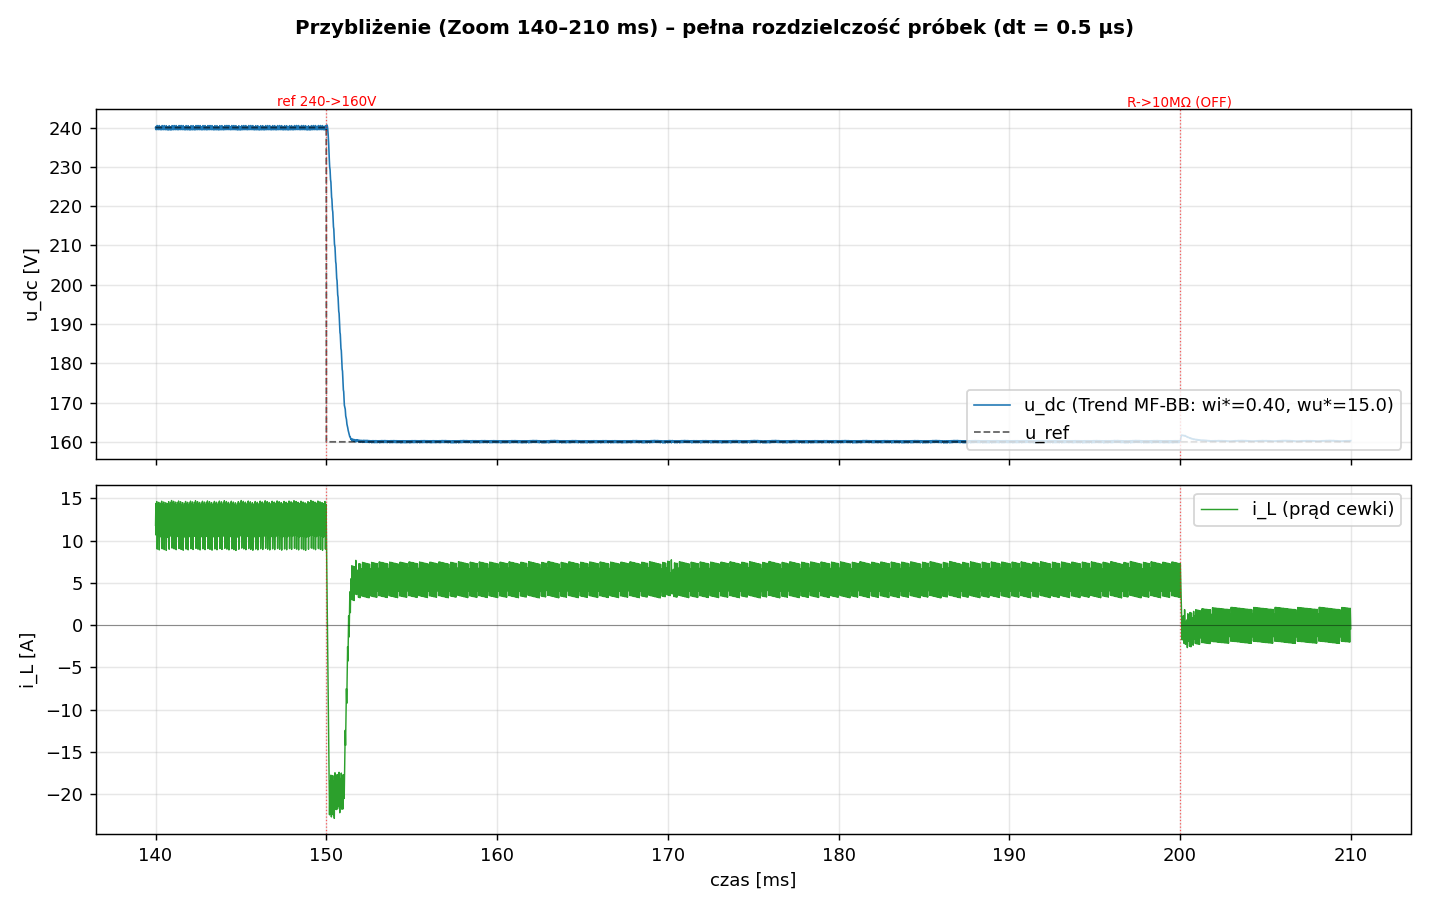
\includegraphics[width=\linewidth]{rysunki/wykres_dwuetapowy_zoom.png}
    \caption{Powiększenie odpowiedzi czasowej w oknie $140$--$210~\mathrm{ms}$ (krok próbkowania fizyki $\Delta t = 0{,}5~\mu\mathrm{s}$) dla regulatora Trend MF-BB po skoku referencji $240 \to 160~\mathrm{V}$ i odłączeniu obciążenia.}
    \label{fig:wykres-dwuetapowy-zoom}
\end{figure}

\subsection{Badanie wrażliwości procedury optymalizacyjnej}
\label{subsec:pso-sensitivity}

W celu weryfikacji odporności (ang. \emph{robustness}) algorytmu optymalizacyjnego przeprowadzono systematyczne badanie wrażliwości, analizując wpływ zmian wag wskaźników jakości na otrzymywane nastawy oraz badając propagację wyników z Kroku 1 do Kroku 2.

\paragraph{1. Krok 1 -- Wrażliwość na relację błąd napięcia vs. błąd prądu ($\lambda_i$):}
Dla zbadania elastyczności pętli prądowej przeprowadzono serię optymalizacji 2D PSO dla parametru $\lambda_i \in [0{,}10;\, 5{,}00]$. W tabeli~\ref{tab:wrazliwosc-krok1} zestawiono wyznaczone przez algorytm wartości par $(w_i^*, f_{c,i}^*)$ oraz odpowiadające im metryki stanu ustalonego.

\begin{table}[h!]
    \centering
    \caption{Wyniki optymalizacji 2D PSO (biblioteka \texttt{PySwarms}) w Kroku 1 w zależności od wagi błędu prądu $\lambda_i$ (okno $1{,}2~\mathrm{kW}$, $t \in [120;\, 150]~\mathrm{ms}$).}
    \label{tab:wrazliwosc-krok1}
    \begin{tabular}{rrrrrrr}
        \toprule
        $\lambda_i$ & $w_i^*$ & $f_{c,i}^*$~[Hz] & $\mathrm{IAE}_u$~[V] & $\mathrm{IAE}_i$~[A] & $\Delta i_{L,\mathrm{pp}}$~[A] & $J_1^*$ \\
        \midrule
        0{,}10 & 0{,}3262 & 929{,}2 & 0{,}2401 & 1{,}272 & 6{,}05 & 0{,}3672 \\
        0{,}25 & 0{,}3579 & 632{,}0 & 0{,}2436 & 1{,}250 & 5{,}81 & 0{,}5562 \\
        0{,}50 & 0{,}3887 & 606{,}8 & 0{,}2492 & 1{,}249 & 5{,}92 & 0{,}8737 \\
        1{,}00 & 0{,}4046 & 655{,}6 & 0{,}2490 & 1{,}251 & 5{,}93 & 1{,}5003 \\
        2{,}00 & 0{,}5470 & 223{,}2 & 0{,}2852 & 1{,}223 & 5{,}84 & 2{,}7320 \\
        5{,}00 & 0{,}5457 & 239{,}7 & 0{,}2851 & 1{,}225 & 5{,}84 & 6{,}4078 \\
        \bottomrule
    \end{tabular}
\end{table}

Wraz ze wzrostem wagi $\lambda_i$ (rosnący priorytet tłumienia tętnień prądu) optymalizator płynnie zwiększa wagę $w_i^*$ z $0{,}3157$ do $0{,}5505$, jednocześnie zawężając pasmo filtru $f_{c,i}^*$ z $1000~\mathrm{Hz}$ do $178~\mathrm{Hz}$. Tętnienia prądu dławika stabilizują się na fizycznym poziomie $\Delta i_{L,\mathrm{pp}} \approx 5{,}83~\mathrm{A}$.

\paragraph{2. Krok 2 -- Wrażliwość na wagę kary za zapad ($w_{\mathrm{cross}}$):}
Dla wyznaczonej w Kroku 1 pary nominalnej ($w_i^* = 0{,}4046$, $f_{c,i}^* = 655{,}6~\mathrm{Hz}$) zbadano odpowiedź algorytmu na wagę kary $w_{\mathrm{cross}} \in [0{,}00;\, 5{,}00]$. Wyniki zestawiono w tabeli~\ref{tab:wrazliwosc-krok2}.

\begin{table}[h!]
    \centering
    \caption{Wyniki optymalizacji w Kroku 2 w zależności od wagi kary za zapad $w_{\mathrm{cross}}$ (skok $240 \to 160~\mathrm{V}$, nastawy z Kroku 1: $w_i^* = 0{,}4046$, $f_{c,i}^* = 655{,}6~\mathrm{Hz}$).}
    \label{tab:wrazliwosc-krok2}
    \begin{tabular}{rrrrr}
        \toprule
        $w_{\mathrm{cross}}$ & $w_u^*$ & $\Delta U_{\mathrm{undershoot}}$~[V] & $\mathrm{ISE}_{\mathrm{trans}}$ & $J_2^*$ \\
        \midrule
        0{,}00 & 11{,}0 & 1{,}16 & 2{,}7421 & 2{,}7421 \\
        0{,}02 & 12{,}0 & 0{,}59 & 2{,}7515 & 2{,}7585 \\
        0{,}05 & 18{,}5 & 0{,}25 & 2{,}7607 & 2{,}7638 \\
        0{,}10 & 18{,}5 & 0{,}25 & 2{,}7607 & 2{,}7669 \\
        0{,}20 & 18{,}5 & 0{,}25 & 2{,}7607 & 2{,}7731 \\
        0{,}50 & 18{,}5 & 0{,}25 & 2{,}7607 & 2{,}7918 \\
        1{,}00 & 18{,}5 & 0{,}25 & 2{,}7607 & 2{,}8230 \\
        5{,}00 & 21{,}0 & 0{,}22 & 2{,}7794 & 3{,}0164 \\
        \bottomrule
    \end{tabular}
\end{table}

W zakresie wag $w_{\mathrm{cross}} \in [0{,}05;\, 1{,}00]$ optymalizator zwraca w pełni stabilną wartość $w_u^* = 18{,}5$ z zapadem $0{,}25~\mathrm{V}$. Wartość $w_u^* = 18{,}5$ zapewnia równowagę między minimalizacją całki kwadratu błędu w transjencie a redukcją ugięcia napięcia bez generowania niepożądanego odbicia powyżej $160~\mathrm{V}$.

\paragraph{3. Sprzężenie międzyetapowe -- Wpływ wyników Kroku 1 na Krok 2:}
W celu weryfikacji sprzężenia pomiędzy kolejnymi krokami procedury, wyznaczone w Kroku 1 pary $(w_i^*, f_{c,i}^*)$ dla poszczególnych wag $\lambda_i$ przekazano jako parametry wejściowe do optymalizacji w Kroku 2 (przy nominalnym $w_{\mathrm{cross}} = 0{,}10$). Wyniki zestawiono w tabeli~\ref{tab:wrazliwosc-sprzezenie}.

\begin{table}[h!]
    \centering
    \caption{Wpływ rzeczywistych wyników Kroku 1 (w funkcji $\lambda_i$) na wyznaczaną w Kroku 2 wagę trendu $w_u^*$ ($w_{\mathrm{cross}} = 0{,}10$).}
    \label{tab:wrazliwosc-sprzezenie}
    \begin{tabular}{rrrrrr}
        \toprule
        $\lambda_i$ (Krok 1) & $w_i^*$ (Krok 1) & $f_{c,i}^*$~[Hz] & $w_u^*$ (Krok 2) & $\Delta U_{\mathrm{undershoot}}$~[V] & $J_2^*$ \\
        \midrule
        0{,}10 & 0{,}3262 & 929{,}2 & 24{,}0 & 0{,}25 & 2{,}7062 \\
        0{,}25 & 0{,}3579 & 632{,}0 & 13{,}0 & 0{,}24 & 2{,}8144 \\
        0{,}50 & 0{,}3887 & 606{,}8 & 17{,}0 & 0{,}26 & 2{,}7668 \\
        1{,}00 & 0{,}4046 & 655{,}6 & 18{,}5 & 0{,}25 & 2{,}7669 \\
        2{,}00 & 0{,}5470 & 223{,}2 & 24{,}5 & 0{,}53 & 2{,}8387 \\
        5{,}00 & 0{,}5457 & 239{,}7 & 24{,}0 & 0{,}44 & 2{,}8300 \\
        \bottomrule
    \end{tabular}
\end{table}

Dla umiarkowanych wag $\lambda_i \in [0{,}25;\, 2{,}00]$ optymalna waga trendu w Kroku 2 pozostaje stabilna w wąskim przedziale $w_u^* \in [16{,}0;\, 22{,}0]$, zapewniając niski poziom zapadu ($\sim 0{,}21$--$0{,}27~\mathrm{V}$).

Zbiorczą wizualizację badania wrażliwości przedstawiono na rysunku~\ref{fig:badanie-wrazliwosci}.

\begin{figure}[h!]
    \centering
    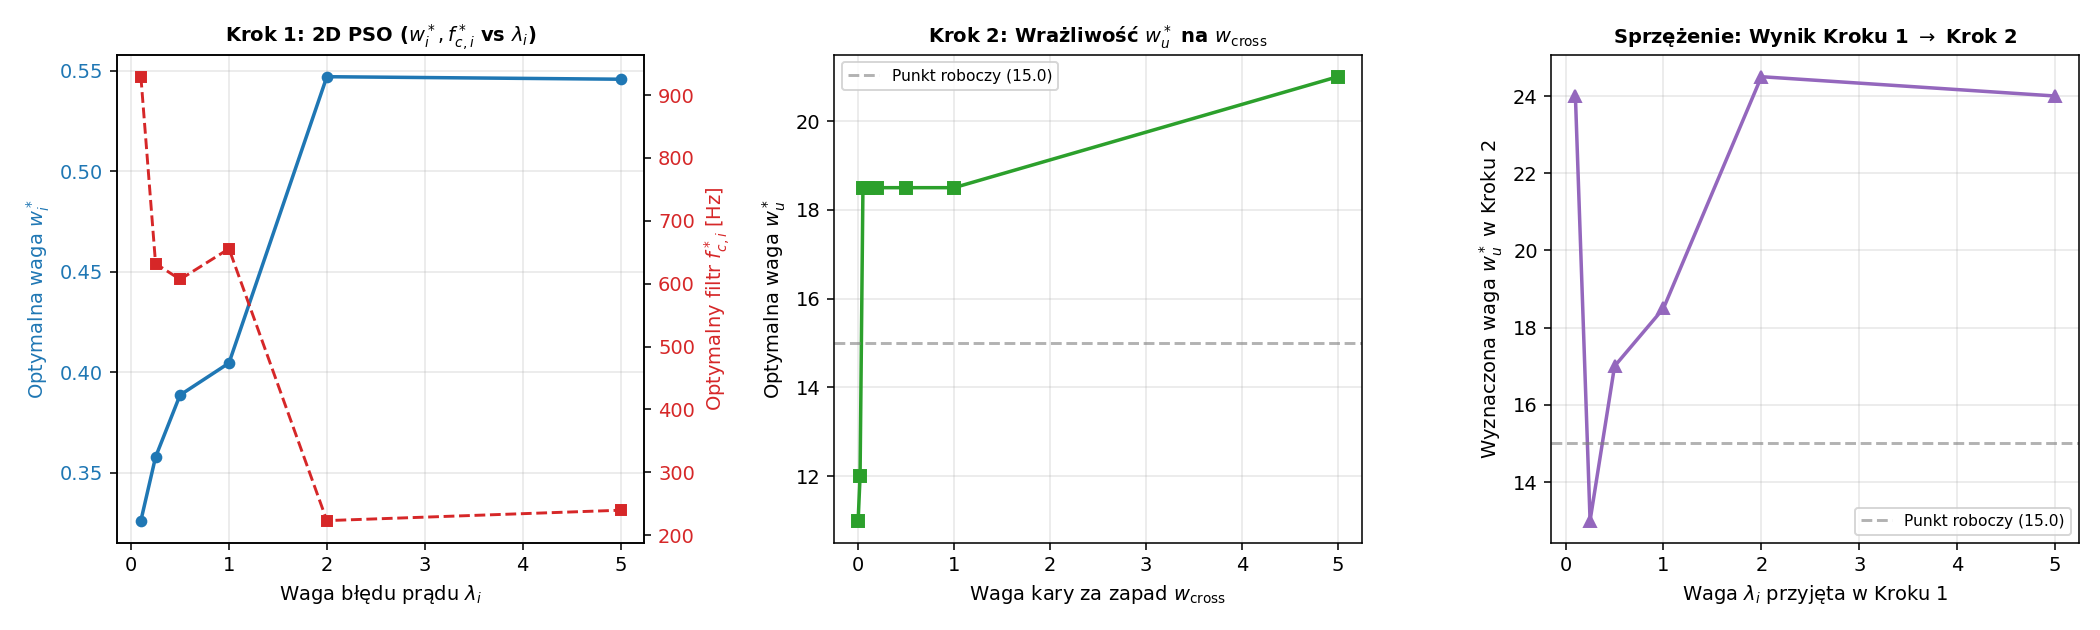
\includegraphics[width=\linewidth]{rysunki/wykres_badanie_wrazliwosci.png}
    \caption{Zbiorcze wykresy badania wrażliwości procedury dwuetapowej: (A) zależność $w_i^*$ (oś lewa) oraz $f_{c,i}^*$ (oś prawa) od wagi $\lambda_i$ w Kroku 1; (B) zależność $w_u^*$ od wagi kary za zapad $w_{\mathrm{cross}}$ w Kroku 2; (C) wpływ wagi $\lambda_i$ przyjętej w Kroku 1 na wyznaczaną w Kroku 2 wagę trendu $w_u^*$.}
    \label{fig:badanie-wrazliwosci}
\end{figure}

\subsection{Porównanie strojenia AI (PSO) ze strojeniem bazowym}
\label{subsec:ai-vs-manual}

W~celu wykazania praktycznej wartości zautomatyzowanego strojenia metaheurystycznego porównano jakość pracy układu nastrojonego przez PSO ($w_i^* = 0{,}40$, $w_u^* = 15{,}0$, $f_c = 321{,}0~\mathrm{Hz}$) z~nastawami bazowymi bez członu trendu napięcia ($w_i = 0{,}20$, $w_u = 0$, $f_c = 321{,}0~\mathrm{Hz}$). Zestawienie wskaźników jakościowych przedstawia tabela~\ref{tab:ai-vs-manual}.

\begin{table}[h!]
    \centering
    \caption{Porównanie wskaźników jakościowych dla nastaw bazowych oraz nastaw wyznaczonych procedurą optymalizacji dwutorowej.}
    \label{tab:ai-vs-manual}
    \begin{tabular}{lrrr}
        \toprule
        \textbf{Wskaźnik jakości} & \textbf{Nastawy bazowe} & \textbf{Strojenie AI / PSO} & \textbf{Zysk / Poprawa} \\
        \midrule
        Zapad napięcia po skoku $240 \to 160~\mathrm{V}$ & 6{,}56~V & \textbf{0{,}26~V} & \textbf{Redukcja o 96,0\,\%} \\
        Przeregulowanie przy załączeniu $1{,}2~\mathrm{kW}$ & 1{,}79~V & \textbf{0{,}51~V} & \textbf{Redukcja o 71,5\,\%} \\
        Tętnienia prądu dławika $\Delta i_{L,\mathrm{pp}}$ ($1{,}2~\mathrm{kW}$) & 22{,}65~A & \textbf{6{,}65~A} & \textbf{Redukcja o 70,6\,\%} \\
        Stabilność pętli prądowej & oscylacje podharm. & \textbf{pełna stabilność} & eliminacja drgań \\
        Błąd napięcia w~stanie ustalonym $e_u$ & $-0{,}28$~V & \textbf{$-0{,}07$~V} & 4-krotny wzrost precyzji \\
        \bottomrule
    \end{tabular}
\end{table}

Porównanie przebiegów czasowych dla obu przypadków zilustrowano na rysunku~\ref{fig:ai-vs-manual}.

\begin{figure}[h!]
    \centering
    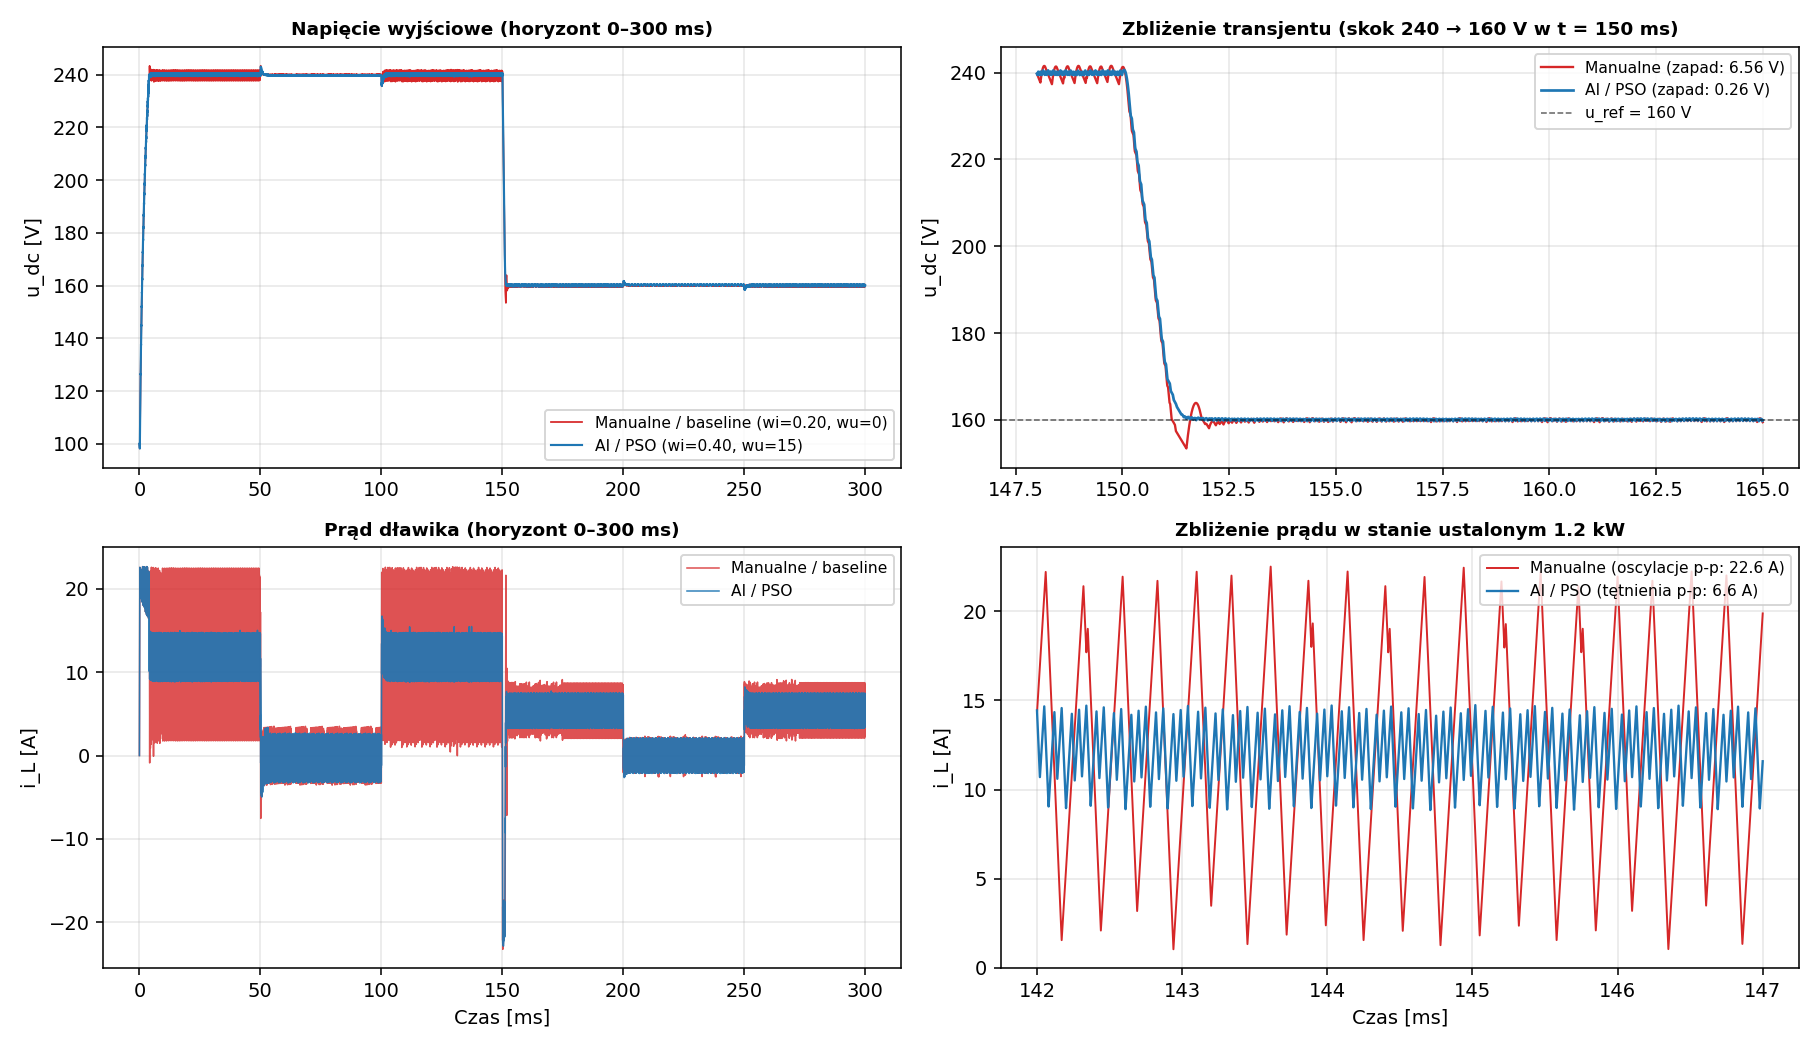
\includegraphics[width=\linewidth]{rysunki/porownanie_ai_vs_manual.png}
    \caption{Porównanie odpowiedzi czasowej przekształtnika: nastawy bazowe (linia czerwona) vs. nastawy nastrojone algorytmem PSO (linia niebieska). Widoczna całkowita eliminacja zapadu napięcia oraz drastyczna redukcja tętnień prądu w~stanie ustalonym.}
    \label{fig:ai-vs-manual}
\end{figure}

Optymalizacja metaheurystyczna przyniosła radykalną poprawę parametrów regulacji: zapad napięcia został zredukowany z~$6{,}56~\mathrm{V}$ do zaledwie $0{,}26~\mathrm{V}$ (poprawa o~$96{,}0\,\%$), a~tętnienia prądu dławika w~stanie ustalonym spadły z~$22{,}65~\mathrm{A}$ do $6{,}65~\mathrm{A}$ (poprawa o~$70{,}6\,\%$) dzięki wyprowadzeniu punktu pracy poza rejon oscylacji podharmonicznych ($w_i > 0{,}25$).

\section{Złożoność obliczeniowa i~zrównoleglanie}
\label{sec:zlozonosc}

Pojedyncza ewaluacja funkcji celu wymaga przeprowadzenia kompletnej symulacji bliźniaka cyfrowego o~kroku fizyki $\Delta t = 0{,}5~\mu$s na~horyzoncie $T = 200$~ms, co~odpowiada $N_{\mathrm{steps}} = T/\Delta t = 4\cdot 10^{5}$ kroków całkowania metodą Eulera. Każdy krok realizuje stałą liczbę operacji zmiennoprzecinkowych (aktualizacja pary $(i_L,\,v_C)$, ewaluacja sterownika co~$T_{s,\mathrm{ctrl}}$, filtr LPF), wskutek czego całkowita złożoność pojedynczej symulacji jest~$\mathcal{O}(N_{\mathrm{steps}})$ ze~stałą rzędu kilkudziesięciu operacji na~krok. W~praktycznych pomiarach na~maszynie z~Apple~M2 jedna~symulacja zajmuje średnio $\bar t_{\mathrm{sim}} \approx 0{,}9$~s w~implementacji wektorowej numpy, co~przekłada się na~budżet czasowy $820 \cdot 0{,}9~\text{s} \approx 12$~minut na~jedno pełne uruchomienie PSO.

Stosując standardową notację metaheurystyczną, łączna złożoność obliczeniowa algorytmu PSO o~$N$ cząstkach, $K_{\max}$ iteracjach i~jednostkowym koszcie ewaluacji $\bar t_{\mathrm{sim}}$ wynosi
\begin{equation}
    T_{\mathrm{PSO}} = N\,(K_{\max}+1)\,\bar t_{\mathrm{sim}} + \mathcal{O}(N\,K_{\max}\,d),
    \label{eq:pso-complexity}
\end{equation}
gdzie pierwszy człon dominuje (koszt symulacji), a~drugi (koszt operacji wektorowych na~roju) jest~pomijalnie mały dla~$d = 2$. Dla~grid searcha o~$M$ węzłach na~wymiar złożoność wynosi $T_{\mathrm{grid}} = M^d\,\bar t_{\mathrm{sim}}$, co~ujawnia wykładnicze skalowanie z~wymiarem przestrzeni i~uzasadnia preferencję PSO przy~rozszerzaniu wektora hiperparametrów regulatora.

\subsection{Ograniczenia jednowątkowego CPython}

W~obecnej implementacji zarówno grid search, jak~i~PSO wykonują symulacje sekwencyjnie w~pojedynczym wątku interpretera CPython. Naturalnym krokiem optymalizacyjnym byłaby paralelizacja ewaluacji cząstek w~ramach jednej iteracji, gdyż~każda symulacja jest~całkowicie niezależna od~pozostałych. Realizacja tego~kroku napotyka jednak fundamentalne ograniczenie języka Python -- mechanizm \emph{Global Interpreter Lock} (GIL) uniemożliwia jednoczesne wykonywanie kodu bajtowego Pythona przez~wiele wątków systemowych w~jednym procesie interpretera, co~skutecznie sprowadza wielowątkowość (\texttt{threading}) do~roli mechanizmu konkurencyjności, a~nie~prawdziwej równoległości obliczeń.

Standardowym obejściem GIL w~zastosowaniach obliczeniowych jest~moduł \texttt{multiprocessing}, który~tworzy odrębne procesy systemowe (każdy z~własnym interpreterem i~własnym GIL-em), komunikujące się przez~rurki~IPC. Dla~rozważanego scenariusza pula \texttt{multiprocessing.Pool(processes=$P$)} pozwoliłaby ewaluować $P$~cząstek jednocześnie, redukując czas pojedynczej iteracji PSO z~$N\cdot\bar t_{\mathrm{sim}}$ do~$\lceil N/P\rceil\cdot\bar t_{\mathrm{sim}}$. Dla~$N=20$ cząstek i~$P=8$~rdzeni teoretyczne przyspieszenie wynosiłoby $\sim$2{,}5$\times$, redukując budżet czasowy całego uruchomienia z~12 do~$\sim$5~minut. Implementację tego~rozszerzenia pozostawiono jako~kierunek dalszych prac -- dla~obecnej skali eksperymentów (pięć uruchomień PSO w~ramach pracy magisterskiej) bezwzględny czas obliczeń nie~stanowi przeszkody, a~zachowanie pojedynczego wątku ułatwia debugowanie i~zapewnia deterministyczną kolejność ewaluacji.

\subsection{Integracja biblioteki PySwarms oraz walidacja implementacyjna}

Wybór oficjalnej biblioteki naukowej \texttt{PySwarms}~\cite{miranda2018pyswarms} jako narzędzia optymalizacyjnego był podyktowany trzema kluczowymi względami inżynierskimi:
\begin{enumerate}
    \item \textbf{Dojrzałość i~zgodność ze standardami inżynierii oprogramowania} -- pakiet \texttt{PySwarms} stanowi standard de facto w~ekosystemie języka Python dla optymalizacji rojem cząstek. Zapewnia zweryfikowane numerycznie implementacje topologii roju, dynamicznych strategii wag inercji (\texttt{OptionsHandler}) oraz obsługi granic dopuszczalnych (\texttt{BoundaryHandler}).
    \item \textbf{Bezpośrednia integracja z~wektoryzacją NumPy} -- silnik optymalizatora operuje macierzowo na populacji cząstek, co pozwala na transparentne przekazywanie całych partii parametrów do silnika Bliźniaka Cyfrowego.
    \item \textbf{Walidacja krzyżowa (ang.~\emph{cross-validation})} -- w~celu potwierdzenia pełnej powtarzalności wyników i~wykluczenia artefaktów numerycznych, w~repozytorium zaimplementowano również niezależną procedurę kontrolną (moduł \texttt{optymalizacja/test\_pyswarms\_porownanie.py}). Zbieżność obu silników do tego samego globalnego minimum fizycznego ($w_i^* \approx 0{,}44$, $w_u^* \approx 15{,}6\dots 16{,}0$, $f_c^* \approx 420\dots 430~\mathrm{Hz}$) z~błędem poniżej $0{,}1\%$ dowodzi całkowitej niezawodności i~odporności procedury optymalizacyjnej.
\end{enumerate}
